\documentclass{beamer}

\usepackage{epsfig}
\usepackage{multicol}
\usepackage{geometry}
%\usepackage[dvipsnames]{xcolor}
\usepackage{textcomp}
\usepackage{graphicx}
\usepackage{caption}
\usepackage{subcaption}
\usepackage{amsmath}
\usepackage{tcolorbox}
\usetheme{Boadilla}
\usepackage{pict2e}
\usepackage{tikz}
\usepackage{xcolor}


\title[Traitement du signal numérique]{Traitement du signal numérique - HEI4 IMS}
\author[Antony Bazir]{}

\setlength{\unitlength}{1cm}

\begin{document}


\section{Filtres numériques: Synthèses et mise en oeuvre}
\subsection{Introduction}
\begin{frame}
\frametitle{Introduction}
Dans la section précédente on a étudie un filtre récursif et un filtre non récursif \\
\vspace{0.3cm}

\begin{columns}

\column{60mm}
\only<2->{
\begin{center}
	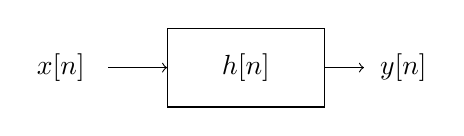
\begin{tikzpicture}
	\draw (2.15,0) node {$x[n]$};
	
	\draw[->] (2.75,0)-- (3.5,0);
	\draw (3.5,-0.5) rectangle(5.5,0.5) ;
	\draw (4.5,0) node {$h[n]$};
	
	\draw[->] (5.5,0)-- (6,0);

	\draw (6.5,0) node {$y[n]$};
	%\draw (4.5,-2) node {filtre non-récursif};
\end{tikzpicture}
\end{center}
}

\column{60mm}
\only<2->{
\begin{center}
	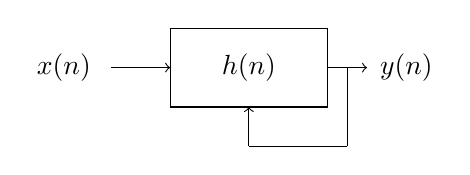
\begin{tikzpicture}
	\draw (2.15,0) node {$x(n)$};

	
	\draw[->] (2.75,0)-- (3.5,0);
	\draw (3.5,-0.5) rectangle(5.5,0.5) ;
	\draw (4.5,0) node {$h(n)$};
	
	\draw[->] (5.5,0)-- (6,0); 
	\draw (6.5,0) node {$y(n)$};

	%\draw (4.5,-2) node {filtre récursif};
	
	\draw[-] (5.75,0)-- (5.75,-1);
	\draw[-] (5.75,-1)-- (4.5,-1);
	\draw[->] (4.5,-1)-- (4.5,-0.5);
	\end{tikzpicture}
\end{center}

}

\end{columns}
%\phantom{.\\}
\vspace{1.3cm}
\only<3->{
On a étudié les propriétés de filtres existants mais on ne sait pas comment les "fabriquer" \only<4->{$\rightarrow$ Synthèse de filtre}
}

\end{frame}


\begin{frame}
\frametitle{Introduction}
Les méthodes de synthèse pour les filtres récursifs et non récursifs sont assez différentes...\\
\vspace{0.3cm}

\begin{columns}

\column{60mm}
\begin{center}
	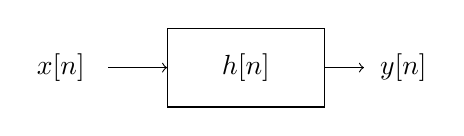
\begin{tikzpicture}
	\draw (2.15,0) node {$x[n]$};
	
	\draw[->] (2.75,0)-- (3.5,0);
	\draw (3.5,-0.5) rectangle(5.5,0.5) ;
	\draw (4.5,0) node {$h[n]$};
	
	\draw[->] (5.5,0)-- (6,0);

	\draw (6.5,0) node {$y[n]$};
	%\draw (4.5,-2) node {filtre non-récursif};
\end{tikzpicture}
\end{center}
\only<2->{
Objectif : calculer les \textbf{coefficients de la réponse impulsionnelles} qui correspondent au gabarit
}

\column{60mm}
\begin{center}
	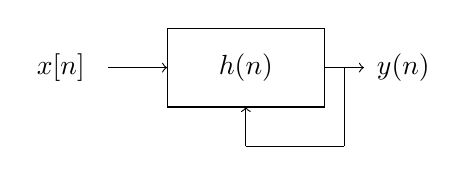
\begin{tikzpicture}
	\draw (2.15,0) node {$x[n]$};

	
	\draw[->] (2.75,0)-- (3.5,0);
	\draw (3.5,-0.5) rectangle(5.5,0.5) ;
	\draw (4.5,0) node {$h(n)$};
	
	\draw[->] (5.5,0)-- (6,0); 
	\draw (6.5,0) node {$y(n)$};

	%\draw (4.5,-2) node {filtre récursif};
	
	\draw[-] (5.75,0)-- (5.75,-1);
	\draw[-] (5.75,-1)-- (4.5,-1);
	\draw[->] (4.5,-1)-- (4.5,-0.5);
	\end{tikzpicture}
\end{center}

\only<2->{
Objectif : \textbf{discrétiser un filtre continu} qui corresponde au gabarit
}

\end{columns}
\end{frame}

\subsection{Synthèse de filtres non-récursifs:  \'Etude filtre passe-bas idéal}
\subsubsection{Réponse impulsionnelle idéale}
\begin{frame}
On commence par les \textbf{filtres non-récursifs}\\
\frametitle{Premier exemple :  Filtre passe-bas idéal}

\vspace{0.3cm}
synthèse de filtre : Passe-bas idéal\\
\vspace{0.3cm}
\begin{columns}

\column{60mm}
\begin{center}
\begin{tikzpicture}

	\draw[->] (-0.5,0)-- (3.5,0);
\draw (-0.3,-0.3) node {0};
\draw[->] (0,0)-- (0,3);
\draw (3.6,0.25) node {$f$};
\draw (0,3.5) node {$|H(f)|$};
\only<1>{
\draw (1,-0.3) node {$f_1$};
\draw (2,-0.3) node {$f_2$};
\draw (-0.6,1.7) node {$1 - \delta_1$};
\draw (-0.6,2.3) node {$1 + \delta_1$};
\draw (-0.3,0.3) node {$\delta_2$};
}
\draw (3,-0.3) node {$f_e/2$};

\only<1>{
\draw[thick,blue](0,1.7)--(1,1.7)--(1,0);
\draw[thick,blue](0,2.3)--(1,2.3)--(1,3);
\draw[thick,blue](2,3)--(2,0.3)--(3,0.3);
}

\only<2->{
\draw[dashed,blue](0,1.7)--(1,1.7)--(1,0);
\draw[dashed,blue](0,2.3)--(1,2.3)--(1,3);
\draw[dashed,blue](2,3)--(2,0.3)--(3,0.3);
}

\only<2->{
	\draw[thick,red]   (0,2)--(1.5,2)--(1.5,0)--(3,0);
	\draw (1.5,-0.3) node {$f_e/4$};
}

\end{tikzpicture}
\end{center}

\column{60mm}
\only<3->{
Ce filtre va correspondre à une réponse impulsionnelle...\\
\vspace{0.5cm}
Comment l'obtenir ?

\begin{itemize} 
\item<4-> Transformée en Z inverse ? \only<5->{ Non... Trop compliqué} 
\item<6-> Développer en série de Fourier
\item<7-> Calculer la fonction continue connue et échantillonner
\end{itemize} 

}

\end{columns}

\end{frame}


\begin{frame}
\frametitle{Premier exemple :  Filtre passe-bas idéal}

\vspace{0.3cm}
Pour comprendre les défis de la synthèse de filtre : Passe-bas idéal\\
\vspace{0.3cm}
\begin{columns}

\column{60mm}
\begin{center}
\begin{tikzpicture}

	\draw[->] (-0.5,0)-- (3.5,0);
\draw (-0.3,-0.3) node {0};
\draw[->] (0,0)-- (0,3);
\draw (3.6,0.25) node {$f$};
\draw (0,3.5) node {$|H(f)|$};

\draw (3,-0.3) node {$f_e/2$};


\draw[dashed,blue](0,1.7)--(1,1.7)--(1,0);
\draw[dashed,blue](0,2.3)--(1,2.3)--(1,3);
\draw[dashed,blue](2,3)--(2,0.3)--(3,0.3);

	\draw[thick,red]   (0,2)--(1.5,2)--(1.5,0)--(3,0);
	\draw (1.5,-0.3) node {$f_e/4$};

\end{tikzpicture}
\end{center}

\column{60mm}
Développement en série de Fourier ? \\
\vspace{0.1cm}
\begin{itemize}
\item<2-> Spectre jusqu'à $f_e/2$ $\rightarrow$ signal discret
\vspace{0.1cm}
\item<3-> Signal discret  $f_e/2$ $\rightarrow$ spectre périodique
\vspace{0.1cm}
\item<4-> Spectre périodique  $f_e/2$ $\rightarrow$ spectre développable en série de fourier 
\vspace{0.1cm}
\item<5-> Coefficients de fourier d'une fct°  $f_e/2$ $\rightarrow$ réponse impulsionnelle discrète...
\end{itemize}

\end{columns}

\end{frame}

\begin{frame}
\frametitle{Premier exemple :  Filtre passe-bas idéal}


\vspace{0.3cm}
Pour comprendre les défis de la synthèse de filtre : Passe-bas idéal\\
\vspace{0.3cm}
\begin{columns}

\column{60mm}
\begin{center}
\begin{tikzpicture}

	\draw[->] (-0.5,0)-- (3.5,0);
\draw (-0.3,-0.3) node {0};
\draw[->] (0,0)-- (0,3);
\draw (3.6,0.25) node {$f$};
\draw (0,3.5) node {$|H(f)|$};

\draw (3,-0.3) node {$f_e/2$};


\draw[dashed,blue](0,1.7)--(1,1.7)--(1,0);
\draw[dashed,blue](0,2.3)--(1,2.3)--(1,3);
\draw[dashed,blue](2,3)--(2,0.3)--(3,0.3);

	\draw[thick,red]   (0,2)--(1.5,2)--(1.5,0)--(3,0);
	\draw (1.5,-0.3) node {$f_e/4$};

\end{tikzpicture}
\end{center}

\column{60mm}
Réponse impulsionnelle continue + échantillonnage ? \\
\vspace{0.1cm}
\begin{itemize}
\item<2-> Spectre jusqu'à $f_e/2$ $\rightarrow$ Spectre jusqu'à $+ \infty$
\vspace{0.1cm}
\item<3-> TF inverse sur spectre $\rightarrow$ Signal temporel continu 
\vspace{0.1cm}
\item<4-> Signal temporel continu  $\rightarrow$ Signal échantillonné à $f_e$
\vspace{0.1cm}
\end{itemize}

\end{columns}
\end{frame}

\begin{frame}
\frametitle{Premier exemple :  Filtre passe-bas idéal}
Résultat des 3 méthodes:\\
\vspace{0.3cm}
\begin{columns}

\column{60mm}
Réponse en fréquence :\\
\vspace{0.2cm}
\begin{center}
\begin{tikzpicture}

	\draw[->] (-0.5,0)-- (3.5,0);
\draw (-0.3,-0.3) node {0};
\draw[->] (0,0)-- (0,3);
\draw (3.6,0.25) node {$f$};
\draw (0,3.5) node {$|H(f)|$};

\draw (3,-0.3) node {$f_e/2$};


\draw[dashed,blue](0,1.7)--(1,1.7)--(1,0);
\draw[dashed,blue](0,2.3)--(1,2.3)--(1,3);
\draw[dashed,blue](2,3)--(2,0.3)--(3,0.3);

	\draw[thick,red]   (0,2)--(1.5,2)--(1.5,0)--(3,0);
	\draw (1.5,-0.3) node {$f_e/4$};
	
	\draw[->] (3.5,2)--(6.5,2);

\end{tikzpicture}
\end{center}

\column{60mm}
Réponse impulsionnelle échantillonnée correspondante:\\
\vspace{0.2cm}

\begin{center}
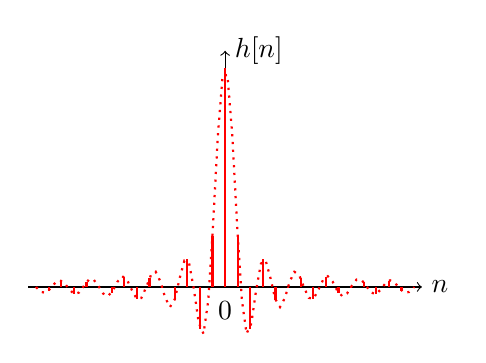
\begin{tikzpicture}
\draw[->] (-2.5,0)-- (2.5,0) node[right]{$n$};
\draw (0,-0.3) node {0};
\draw[->] (0,0)-- (0,3)node[right]{$h[n]$};

\draw[dotted,thick, domain=-2.4:2.4,color=red,samples=80] plot (\x,{160*sin(5*3.14*\x r  )/(5*3.14*\x r)});
\draw[thick, domain=-2.4:2.4,color=red,samples=31] plot [ycomb] (\x,{160*sin(5*3.14*\x r  )/(5*3.14*\x r)});


\end{tikzpicture}
\end{center}
\vspace{0.3cm}
\[ h[n] = \frac{\sin(\pi nT_e)}{\pi n T_e} \]

\end{columns}

\end{frame} 

\subsubsection{Réponse impulsionnelle réelle : fenêtrage}
\begin{frame}
\frametitle{Premier exemple :  Filtre passe-bas idéal} 
\textbf{PROBL\`EME !!!}

\begin{columns}
\column{60mm}
\begin{center}
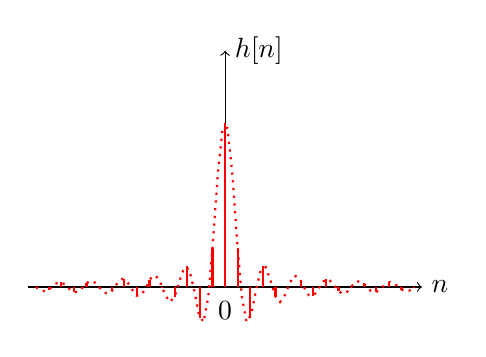
\begin{tikzpicture}
\draw[->] (-2.5,0)-- (2.5,0) node[right]{$n$};
\draw (0,-0.3) node {0};
\draw[->] (0,0)-- (0,3)node[right]{$h[n]$};

\draw[dotted,thick, domain=-2.4:2.4,color=red,samples=80] plot (\x,{120*sin(5*3.14*\x r  )/(5*3.14*\x r)});
\draw[thick, domain=-2.4:2.4,color=red,samples=31] plot [ycomb] (\x,{120*sin(5*3.14*\x r  )/(5*3.14*\x r)});


\end{tikzpicture}
\end{center}

\column{60mm}

\only<2->{
La réponse impulsionnelle est \textbf{infinie}\\
\vspace{1cm}

}

\only<3->{
On ne peut pas coder cette fonction sur un support numérique...
}

\end{columns}
\end{frame}

\begin{frame}
\frametitle{Premier exemple :  Filtre passe-bas idéal} 

\begin{columns}
\column{60mm}
\begin{center}
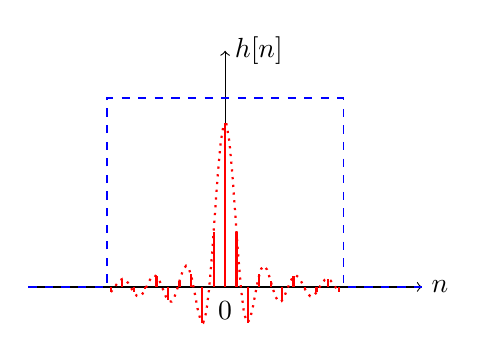
\begin{tikzpicture}
\draw[->] (-2.5,0)-- (2.5,0) node[right]{$n$};
\draw (0,-0.3) node {0};
\draw[->] (0,0)-- (0,3)node[right]{$h[n]$};

\draw[dotted,thick, domain=-1.45:1.45,color=red,samples=80] plot (\x,{120*sin(5*3.14*\x r  )/(5*3.14*\x r)});
\draw[thick, domain=-1.45:1.45,color=red,samples=21] plot [ycomb] (\x,{120*sin(5*3.14*\x r  )/(5*3.14*\x r)});

\only<2->{
		\draw[dashed,blue] (-2.5,0)--(-1.5,0)--(-1.5,2.4)--(1.5,2.4)--(1.5,0)--(2.5,0);
}


\end{tikzpicture}
\end{center}

\column{60mm}
Il faut un nombre \textbf{fini} d'échantillon\\
\vspace{1cm}
\only<2->{
$\rightarrow$ Application d'une \textbf{fenêtre temporelle}.
\\}
\vspace{1cm}
\only<3->{
Effet de l'application de la fenêtre sur la réponse en fréquence ?
}

\end{columns}
\end{frame}

\begin{frame}
\frametitle{Premier exemple :  Filtre passe-bas idéal} 

\begin{columns}
\column{50mm}
\begin{center}
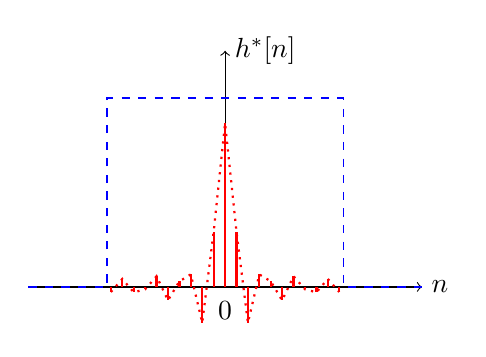
\begin{tikzpicture}
\draw[->] (-2.5,0)-- (2.5,0) node[right]{$n$};
\draw (0,-0.3) node {0};
\draw[->] (0,0)-- (0,3)node[right]{$h^*[n]$};

\draw[dotted,thick, domain=-1.45:1.45,color=red,samples=21] plot (\x,{120*sin(5*3.14*\x r  )/(5*3.14*\x r)});
\draw[thick, domain=-1.45:1.45,color=red,samples=21] plot [ycomb] (\x,{120*sin(5*3.14*\x r  )/(5*3.14*\x r)});


		\draw[dashed,blue] (-2.5,0)--(-1.5,0)--(-1.5,2.4)--(1.5,2.4)--(1.5,0)--(2.5,0);
\end{tikzpicture}
\end{center}

\column{70mm}

Effet de l'application de la fenêtre sur la réponse en fréquence ?\\
\vspace{0.5cm}
\[ h^*[n] = \frac{\sin(\pi nT_e)}{\pi n T_e}\cdot \Pi_M[n]  \]\\
\vspace{0.5cm}
\only<1>{\[ H^*(f) = ?  \]}
\only<2->{\[\boxed{ H^*(f) = TF(\frac{\sin(\pi nT_e)}{\pi n T_e}) \star TF(\Pi_M[n])}  \]}



\end{columns}
\end{frame}

\begin{frame}
\frametitle{Premier exemple :  Filtre passe-bas idéal} 

\begin{columns}[T]
\column{60mm}
\[h^*[n] = \frac{\sin(\pi nT_e)}{\pi n T_e}\cdot \Pi_M[n]\]\\
\vspace{0.5cm}
\begin{center}
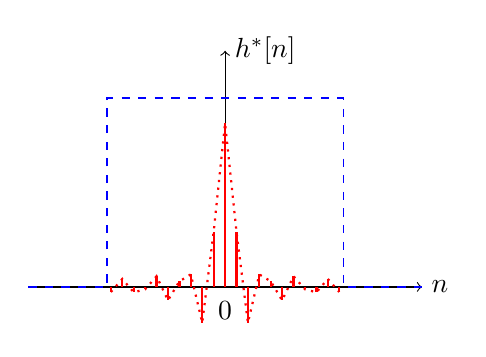
\begin{tikzpicture}
\draw[->] (-2.5,0)-- (2.5,0) node[right]{$n$};
\draw (0,-0.3) node {0};
\draw[->] (0,0)-- (0,3)node[right]{$h^*[n]$};

\draw[dotted,thick, domain=-1.45:1.45,color=red,samples=21] plot (\x,{120*sin(5*3.14*\x r  )/(5*3.14*\x r)});
\draw[thick, domain=-1.45:1.45,color=red,samples=21] plot [ycomb] (\x,{120*sin(5*3.14*\x r  )/(5*3.14*\x r)});


		\draw[dashed,blue] (-2.5,0)--(-1.5,0)--(-1.5,2.4)--(1.5,2.4)--(1.5,0)--(2.5,0);
\end{tikzpicture}
\end{center}

\column{60mm}
\[ H^*(f) = TF(\frac{\sin(\pi nT_e)}{\pi n T_e}) \star TF(\Pi_M[n]) \]\\
\vspace{0.3cm}
\begin{center}
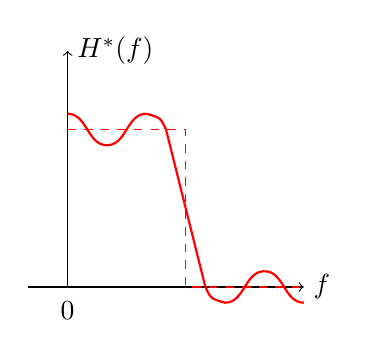
\begin{tikzpicture}

	\draw[->] (-0.5,0)-- (3,0)node[right] {$f$};
\draw (0,-0.3) node {0};
\draw[->] (0,0)-- (0,3) node[right] {$H^*(f)$};


\draw[dashed,red]   (0,2)--(1.5,2)--(1.5,0)--(3,0);

%ondulations BP
 \draw[thick,red] (0,2.2) .. controls (0.25,2.2)  and (0.25,1.8)  .. (0.5,1.8);
  \draw[thick,red] (0.5,1.8) .. controls (0.75,1.8)  and (0.75,2.2)  .. (1,2.2);
   \draw[thick,red] (1,2.2) .. controls (1.18,2.15) and (1.18,2.15)  .. (1.25,2);


%(1.5,2.1) and (1.2,2.1) 

%droite descendant de 1 à 0
\draw[thick,red] (1.25,2)--(1.75,0);

%ondulations BA
  \draw[thick,red] (2,-0.2) .. controls (2.25,-0.2)  and (2.25,0.2)  .. (2.5,0.2);
 \draw[thick,red] (2.5,0.2) .. controls (2.75,0.2)  and (2.75,-0.2)  .. (3,-0.2);
    \draw[thick,red] (1.75,0) .. controls (1.82,-0.15) and (1.82,-0.15)  .. (2,-0.2);


\end{tikzpicture}
\end{center}

\end{columns}

\begin{block}{}
Limitation du nombre de termes $\rightarrow$  Ondulations dans la fonction de transfert
\end{block}

\end{frame}

\begin{frame}
\frametitle{Premier exemple :  Filtre passe-bas idéal} 

\begin{columns}[T]
\column{45mm}
\begin{center}
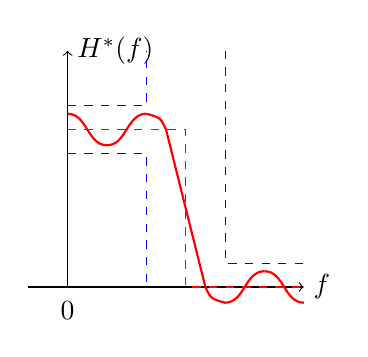
\begin{tikzpicture}

	\draw[->] (-0.5,0)-- (3,0)node[right] {$f$};
\draw (0,-0.3) node {0};
\draw[->] (0,0)-- (0,3) node[right] {$H^*(f)$};


\draw[dashed,red]   (0,2)--(1.5,2)--(1.5,0)--(3,0);

%ondulations BP
 \draw[thick,red] (0,2.2) .. controls (0.25,2.2)  and (0.25,1.8)  .. (0.5,1.8);
  \draw[thick,red] (0.5,1.8) .. controls (0.75,1.8)  and (0.75,2.2)  .. (1,2.2);
   \draw[thick,red] (1,2.2) .. controls (1.18,2.15) and (1.18,2.15)  .. (1.25,2);


%(1.5,2.1) and (1.2,2.1) 

%droite descendant de 1 à 0
\draw[thick,red] (1.25,2)--(1.75,0);
    \only<2->{
		
\draw[dashed,blue](0,1.7)--(1,1.7)--(1,0);
\draw[dashed,blue](0,2.3)--(1,2.3)--(1,3);
\draw[dashed,blue](2,3)--(2,0.3)--(3,0.3);
}   
%ondulations BA
  \draw[thick,red] (2,-0.2) .. controls (2.25,-0.2)  and (2.25,0.2)  .. (2.5,0.2);
 \draw[thick,red] (2.5,0.2) .. controls (2.75,0.2)  and (2.75,-0.2)  .. (3,-0.2);
    \draw[thick,red] (1.75,0) .. controls (1.82,-0.15) and (1.82,-0.15)  .. (2,-0.2);
    
%    \only<2->{
%		
%\draw[dashed,blue](0,1.7)--(1,1.7)--(1,0);
%\draw[dashed,blue](0,2.3)--(1,2.3)--(1,3);
%\draw[dashed,blue](2,3)--(2,0.3)--(3,0.3);
%}    
    
    \end{tikzpicture}
\end{center}


\column{75mm}
On résume :
\begin{itemize}
\item<2-> Réponse impulsionnelle du passe-bas idéal ? \only<3->{ sinus cardinal discret (nombre infini de terme)}
\vspace{0.3cm}
\item<4-> Nombre fini de termes rép. imp. $\rightarrow$ application d'une fenêtre rectangulaire
\vspace{0.3cm}
\item<5-> Fenêtrage en temporel $\rightarrow$ Ondulations sur la fonction  de transfert du filtre réel

\end{itemize}
\end{columns}

\end{frame}

\begin{frame}
\frametitle{Premier exemple :  Filtre passe-bas idéal} 
Reprenons le gabarit...
\begin{columns}[T]
\column{45mm}
\begin{center}
\begin{tikzpicture}

	\draw[->] (-0.5,0)-- (3,0)node[right] {$f$};
\draw (0,-0.5) node {0};
\draw[->] (0,0)-- (0,3) node[right] {$H^*(f)$};


\draw[dashed,red]   (0,2)--(1.5,2)--(1.5,0)--(3,0);

%ondulations BP
 \draw[thick,red] (0,2.2) .. controls (0.25,2.2)  and (0.25,1.8)  .. (0.5,1.8);
  \draw[thick,red] (0.5,1.8) .. controls (0.75,1.8)  and (0.75,2.2)  .. (1,2.2);
   \draw[thick,red] (1,2.2) .. controls (1.18,2.15) and (1.18,2.15)  .. (1.25,2);


%(1.5,2.1) and (1.2,2.1) 

%droite descendant de 1 à 0
\draw[thick,red] (1.25,2)--(1.75,0);
    \only<2->{
		
\draw[dashed,blue](0,1.7)--(1,1.7)--(1,0);
\draw[dashed,blue](0,2.3)--(1,2.3)--(1,3);
\draw[dashed,blue](2,3)--(2,0.3)--(3,0.3);
}   
%ondulations BA
  \draw[thick,red] (2,-0.2) .. controls (2.25,-0.2)  and (2.25,0.2)  .. (2.5,0.2);
 \draw[thick,red] (2.5,0.2) .. controls (2.75,0.2)  and (2.75,-0.2)  .. (3,-0.2);
    \draw[thick,red] (1.75,0) .. controls (1.82,-0.15) and (1.82,-0.15)  .. (2,-0.2);
    
    \only<2->{
		
\draw[dashed,blue](0,1.7)--(1,1.7)--(1,0);
\draw[dashed,blue](0,2.3)--(1,2.3)--(1,3);
\draw[dashed,blue](2,3)--(2,0.3)--(3,0.3);
}    
\only<4->{
\draw (1,-0.5) node {$f_1$};
\draw (2,-0.5) node {$f_2$};
\draw (-0.6,1.7) node {$1 - \delta_1$};
\draw (-0.6,2.3) node {$1 + \delta_1$};
\draw (-0.3,0.4) node {$\delta_2$};
}
    \end{tikzpicture}
\end{center}


\column{75mm}
Commentaires:
\begin{itemize}
\item<3-> filtre réel (nombre fini de termes) = \textbf{Oscillations rép. en fréq.}
\vspace{0.3cm}
\item<4-> Oscillations = tolérance en amplitude + largeur de transition
\vspace{0.3cm}
\item<5-> + de termes = - d'oscillations MAIS mémoire et temps de calcul à prendre en compte
\item<6-> \textbf{Ondulations de même amplitude en bande passante et affaiblie...}
\end{itemize}
\end{columns}

\end{frame}

\subsection{ Méthode des fenêtres}

\begin{frame}
\frametitle{Synthèse de filtres non-récursifs: Méthode des fenêtres}

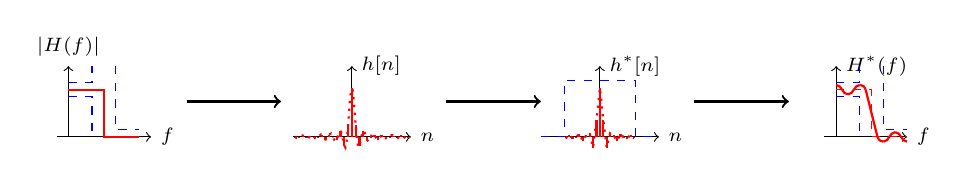
\begin{tikzpicture}
\begin{scope}[scale=0.3]
	\draw[->] (-0.5,0)-- (3.5,0)node[right] {\scriptsize $f$} ;
%\draw (-0.3,-0.3) node {0};
\draw[->] (0,0)-- (0,3)node[above] {\scriptsize $|H(f)|$};


%\draw (3,-0.3) node {$f_e/2$};


\draw[dashed,blue](0,1.7)--(1,1.7)--(1,0);
\draw[dashed,blue](0,2.3)--(1,2.3)--(1,3);
\draw[dashed,blue](2,3)--(2,0.3)--(3,0.3);

	\draw[thick,red]   (0,2)--(1.5,2)--(1.5,0)--(3,0);
	%\draw[->,thick] (0.75,-0.5)--(0.75,-1);
	%\draw (1.5,-0.3) node {$f_e/4$};
	\draw[->,thick] (5,1.5)--(9,1.5);
\end{scope}



\begin{scope}[scale=0.3,xshift=12cm]
%\draw[->,thick] (0,4)--(0,3.4);
\draw[->] (-2.5,0)-- (2.5,0) node[right]{\scriptsize $n$};
%\draw (0,-0.3) node {0};
\draw[->] (0,0)-- (0,3)node[right]{\scriptsize $h[n]$};

\draw[dotted,thick, domain=-2.4:2.4,color=red,samples=80] plot (\x,{120*sin(5*3.14*\x r  )/(5*3.14*\x r)});
\draw[thick, domain=-2.4:2.4,color=red,samples=31] plot [ycomb] (\x,{120*sin(5*3.14*\x r  )/(5*3.14*\x r)});
\draw[->,thick] (4,1.5)--(8,1.5);
\end{scope} 



\begin{scope}[scale=0.3,xshift=22.5cm]
\draw[->] (-2.5,0)-- (2.5,0) node[right]{\scriptsize $n$};
%\draw (0,-0.3) node {0};
\draw[->] (0,0)-- (0,3)node[right]{\scriptsize $h^*[n]$};

\draw[dotted,thick, domain=-1.45:1.45,color=red,samples=21] plot (\x,{120*sin(5*3.14*\x r  )/(5*3.14*\x r)});
\draw[thick, domain=-1.45:1.45,color=red,samples=21] plot [ycomb] (\x,{120*sin(5*3.14*\x r  )/(5*3.14*\x r)});


		\draw[dashed,blue] (-2.5,0)--(-1.5,0)--(-1.5,2.4)--(1.5,2.4)--(1.5,0)--(2.5,0);
		
		\draw[->,thick] (4,1.5)--(8,1.5);
		\end{scope}
		
		%\draw[->,thick] (26,1)--(31,1);
		
		\begin{scope}[scale=0.3,xshift=32.5cm]
	\draw[->] (-0.5,0)-- (3,0)node[right] {\scriptsize $f$};
%\draw (0,-0.5) node {0};
\draw[->] (0,0)-- (0,3) node[right] {\scriptsize $H^*(f)$};


\draw[dashed,red]   (0,2)--(1.5,2)--(1.5,0)--(3,0);

%ondulations BP
 \draw[thick,red] (0,2.2) .. controls (0.25,2.2)  and (0.25,1.8)  .. (0.5,1.8);
  \draw[thick,red] (0.5,1.8) .. controls (0.75,1.8)  and (0.75,2.2)  .. (1,2.2);
   \draw[thick,red] (1,2.2) .. controls (1.18,2.15) and (1.18,2.15)  .. (1.25,2);


%(1.5,2.1) and (1.2,2.1) 

%droite descendant de 1 à 0
\draw[thick,red] (1.25,2)--(1.75,0);
  
\draw[dashed,blue](0,1.7)--(1,1.7)--(1,0);
\draw[dashed,blue](0,2.3)--(1,2.3)--(1,3);
\draw[dashed,blue](2,3)--(2,0.3)--(3,0.3);
 
%ondulations BA
  \draw[thick,red] (2,-0.2) .. controls (2.25,-0.2)  and (2.25,0.2)  .. (2.5,0.2);
 \draw[thick,red] (2.5,0.2) .. controls (2.75,0.2)  and (2.75,-0.2)  .. (3,-0.2);
    \draw[thick,red] (1.75,0) .. controls (1.82,-0.15) and (1.82,-0.15)  .. (2,-0.2);
    
\end{scope}
	

\end{tikzpicture}\\
\vspace{0.5cm}
\textbf{Méthodes de fenêtres} :\\
\vspace{0.2cm}
\begin{enumerate}
\item Réponse en fréquence de filtre idéal 
\vspace{0.2cm}
\item<2-> Réponse impulsionnelle idéale 
\vspace{0.2cm}
\item<3-> Fenêtrage $\rightarrow$ réponse impulsionnelle réelle 
\vspace{0.2cm}
\item<4-> Réponse en fréquence réelle
\end{enumerate}



\end{frame}

\begin{frame}
\frametitle{Synthèse de filtres non-récursifs: Méthode des fenêtres}

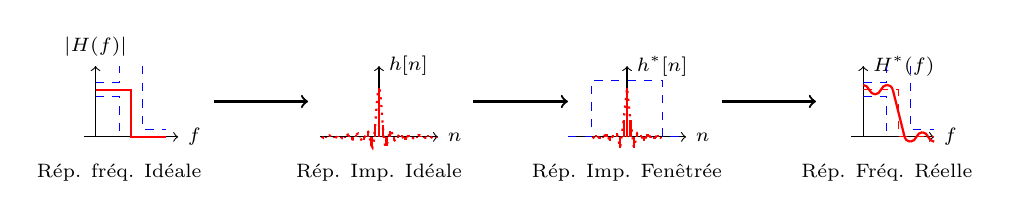
\begin{tikzpicture}
\begin{scope}[scale=0.3]
	\draw[->] (-0.5,0)-- (3.5,0)node[right] {\scriptsize $f$} ;
%\draw (-0.3,-0.3) node {0};
\draw[->] (0,0)-- (0,3)node[above] {\scriptsize $|H(f)|$};


%\draw (3,-0.3) node {$f_e/2$};


\draw[dashed,blue](0,1.7)--(1,1.7)--(1,0);
\draw[dashed,blue](0,2.3)--(1,2.3)--(1,3);
\draw[dashed,blue](2,3)--(2,0.3)--(3,0.3);

	\draw[thick,red]   (0,2)--(1.5,2)--(1.5,0)--(3,0);
	%\draw[->,thick] (0.75,-0.5)--(0.75,-1);
	%\draw (1.5,-0.3) node {$f_e/4$};
	\draw[->,thick] (5,1.5)--(9,1.5);
	\draw (1,-1.5) node[text centered] {\scriptsize Rép. fréq. Idéale};
\end{scope}



\begin{scope}[scale=0.3,xshift=12cm]
%\draw[->,thick] (0,4)--(0,3.4);
\draw[->] (-2.5,0)-- (2.5,0) node[right]{\scriptsize $n$};
%\draw (0,-0.3) node {0};
\draw[->] (0,0)-- (0,3)node[right]{\scriptsize $h[n]$};

\draw[dotted,thick, domain=-2.4:2.4,color=red,samples=80] plot (\x,{120*sin(5*3.14*\x r  )/(5*3.14*\x r)});
\draw[thick, domain=-2.4:2.4,color=red,samples=31] plot [ycomb] (\x,{120*sin(5*3.14*\x r  )/(5*3.14*\x r)});
\draw[->,thick] (4,1.5)--(8,1.5);
	\draw (0,-1.5) node[text centered] {\scriptsize Rép. Imp. Idéale};
\end{scope} 



\begin{scope}[scale=0.3,xshift=22.5cm]
\draw[->] (-2.5,0)-- (2.5,0) node[right]{\scriptsize $n$};
%\draw (0,-0.3) node {0};
\draw[->] (0,0)-- (0,3)node[right]{\scriptsize $h^*[n]$};

\draw[dotted,thick, domain=-1.45:1.45,color=red,samples=21] plot (\x,{120*sin(5*3.14*\x r  )/(5*3.14*\x r)});
\draw[thick, domain=-1.45:1.45,color=red,samples=21] plot [ycomb] (\x,{120*sin(5*3.14*\x r  )/(5*3.14*\x r)});


		\draw[dashed,blue] (-2.5,0)--(-1.5,0)--(-1.5,2.4)--(1.5,2.4)--(1.5,0)--(2.5,0);
		
		\draw[->,thick] (4,1.5)--(8,1.5);
			\draw (0,-1.5) node[text centered] {\scriptsize Rép. Imp. Fenêtrée};
		\end{scope}
		
		%\draw[->,thick] (26,1)--(31,1);
		
		\begin{scope}[scale=0.3,xshift=32.5cm]
	\draw[->] (-0.5,0)-- (3,0)node[right] {\scriptsize $f$};
%\draw (0,-0.5) node {0};
\draw[->] (0,0)-- (0,3) node[right] {\scriptsize $H^*(f)$};


\draw[dashed,red]   (0,2)--(1.5,2)--(1.5,0)--(3,0);

%ondulations BP
 \draw[thick,red] (0,2.2) .. controls (0.25,2.2)  and (0.25,1.8)  .. (0.5,1.8);
  \draw[thick,red] (0.5,1.8) .. controls (0.75,1.8)  and (0.75,2.2)  .. (1,2.2);
   \draw[thick,red] (1,2.2) .. controls (1.18,2.15) and (1.18,2.15)  .. (1.25,2);


%(1.5,2.1) and (1.2,2.1) 

%droite descendant de 1 à 0
\draw[thick,red] (1.25,2)--(1.75,0);
  
\draw[dashed,blue](0,1.7)--(1,1.7)--(1,0);
\draw[dashed,blue](0,2.3)--(1,2.3)--(1,3);
\draw[dashed,blue](2,3)--(2,0.3)--(3,0.3);
 
%ondulations BA
  \draw[thick,red] (2,-0.2) .. controls (2.25,-0.2)  and (2.25,0.2)  .. (2.5,0.2);
 \draw[thick,red] (2.5,0.2) .. controls (2.75,0.2)  and (2.75,-0.2)  .. (3,-0.2);
    \draw[thick,red] (1.75,0) .. controls (1.82,-0.15) and (1.82,-0.15)  .. (2,-0.2);
    \draw (1,-1.5) node[text centered] {\scriptsize Rép. Fréq. Réelle};
\end{scope}
	

\end{tikzpicture}\\
\vspace{0.5cm}
\textbf{Remarques} :\\
\vspace{0.2cm}
\begin{itemize}
\item Plusieurs fenêtres sont possibles (Hamming, Dolf Tchebycheff,...)
\vspace{0.2cm}
\item<2-> Fenêtre $\rightarrow$ Compromis ondulations/largeur bande de transition
\vspace{0.2cm}
\item<3-> Faible largeur transition = Ondulations importantes 
\vspace{0.2cm}
\item<4-> \textbf{Ondulations de même amplitude en bande passante et affaiblie...}
\end{itemize}

\end{frame}

\subsection{Synthèse de filtres non-récursifs: Différentes méthodes}
\begin{frame}
\frametitle{Synthèse de filtres non-récursifs: Différentes méthodes}
Les méthodes suivent toute le même principe général :

\begin{center}
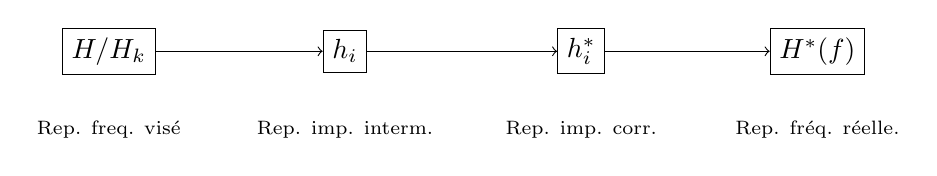
\begin{tikzpicture}
		\node[rectangle,draw,align=center] (I) at (1,0) {$H/H_k$};
		\draw (1,-1) node[text centered] {\scriptsize Rep. freq. visé};
		\node[rectangle,draw,align=center] (D) at (4,0) {$h_i$};
		\draw (4,-1) node[text centered] {\scriptsize Rep. imp. interm.};
		\node[rectangle,draw,align=center] (N) at (7,0) {$h_i^*$};
				\draw (7,-1) node[text centered] {\scriptsize Rep. imp. corr.};
		\node[rectangle,draw,align=center] (B) at (10,0) {$H^*(f)$};	
		\draw (10,-1) node[text centered]{\scriptsize Rep. fréq. réelle.};
		
		\draw[->] (I)--(D);
		\draw[->] (D)--(N);
		\draw[->] (N)--(B);
\end{tikzpicture}
\end{center}

Principales méthodes de synthèse de filtres non-récursifs:
\vspace{0.2cm}
\begin{itemize}
\item<2-> Méthode des fenêtres 
\item<3-> Méthode de l'échantillonnage en fréquence
\item<4-> Méthode des moindres carrés
\item<5-> Méthode par approximation de Tchebychev
\end{itemize}

\end{frame}

\subsection{Méthode de l'échantillonnage en fréquence}
\begin{frame}
\frametitle{Méthode de l'échantillonnage en fréquence}
\begin{columns}
\column{60mm}
\begin{center}
\begin{tikzpicture}
	\draw[->] (-0.5,0)-- (3.5,0)node[right] {\scriptsize $f$} ;
%\draw (-0.3,-0.3) node {0};
\draw[->] (0,0)-- (0,3)node[above] {\scriptsize $H_k$};


%\draw (3,-0.3) node {$f_e/2$};


\draw[dashed,blue](0,1.7)--(1,1.7)--(1,0);
\draw[dashed,blue](0,2.3)--(1,2.3)--(1,3);
\draw[dashed,blue](2,3)--(2,0.3)--(3,0.3);

	%\draw[thick,red]   (0,2)--(1.5,2)--(1.5,0)--(3,0);
	\draw[->,thick,red] (0,0)--(0,2);
	\draw[->,thick,red] (0.5,0)--(0.5,2);
	\draw[->,thick,red] (1,0)--(1,2);
		\draw[->,thick,red] (1.5,0)--(1.5,1);
	\draw[->,thick,red] (2,0)--(2,0);
	\draw[->,thick,red] (2.5,0)--(2.5,0);
	\draw[->,thick,red] (3,0)--(3,0);
\end{tikzpicture}
\end{center}

\column{60mm}
Point départ méthode des fenêtres : Réponse en fréquence idéale continue \\

\vspace{0.5cm}

Point départ Méthode échantillonnage en fréquence : \textbf{Echantillons en fréquence visés}\\
\vspace{0.2cm}
\begin{itemize}
\item<2-> Amplitude des échantillons en bande passante : 1
\item<3-> Amplitude des échantillons en bande passante : 0
\item<4-> Amplitude des échantillons en bande de transition : variable
\end{itemize}

\end{columns}

\end{frame}

\begin{frame}
\frametitle{Méthode de l'échantillonnage en fréquence}
Application de la transformée de Fourier inverse aux $H_k$

\begin{columns}
\column{60mm}
\begin{center}
\begin{tikzpicture}
	\draw[->] (-0.5,0)-- (3.5,0)node[right] {\scriptsize $f$} ;
%\draw (-0.3,-0.3) node {0};
\draw[->] (0,0)-- (0,3)node[above] {\scriptsize $H_k$};


%\draw (3,-0.3) node {$f_e/2$};


\draw[dashed,blue](0,1.7)--(1,1.7)--(1,0);
\draw[dashed,blue](0,2.3)--(1,2.3)--(1,3);
\draw[dashed,blue](2,3)--(2,0.3)--(3,0.3);

	%\draw[thick,red]   (0,2)--(1.5,2)--(1.5,0)--(3,0);
	\draw[->,thick,red] (0,0)--(0,2);
	\draw[->,thick,red] (0.5,0)--(0.5,2);
	\draw[->,thick,red] (1,0)--(1,2);
		\draw[->,thick,red] (1.5,0)--(1.5,1);
	\draw[->,thick,red] (2,0)--(2,0);
	\draw[->,thick,red] (2.5,0)--(2.5,0);
	\draw[->,thick,red] (3,0)--(3,0);
	\draw[->] (4,1.5)--(6,1.5);
	\end{tikzpicture}
\end{center}

\column{60mm}
\begin{center}
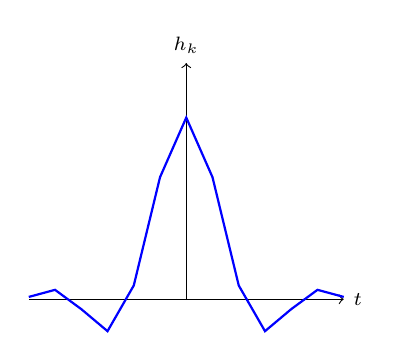
\begin{tikzpicture}
\draw[->] (-2,0)-- (2,0)node[right] {\scriptsize $t$} ;
\draw[->] (0,0)-- (0,3)node[above] {\scriptsize $h_k$};
\draw[thick,blue] plot coordinates{
(-6/3,0.006*5)
(-5/3,0.024*5)
(-4/3,-0.025*5)
(-3/3,-0.081*5)
(-2/3,0.035*5)
(-1/3,0.31*5)
(0/3,0.4615*5)
(1/3,0.31*5)
(2/3,0.035*5)
(3/3,-0.081*5)
(4/3,-0.025*5)
(5/3,0.024*5)
(6/3,0.006*5)};

%\draw[thick,green!20!black] plot coordinates{
%(-6/3,-0.0061*5)
%(-5/3,0.0224*5)
%(-4/3,0.0203*5)
%(-3/3,-0.0538*5)
%(-2/3,-0.0163*5)
%(-1/3,0.0741*5)
%(0,0)
%(1/3,-0.0741*5)
%(2/3,0.0163*5)
%(3/3,0.0538*5)
%(4/3,-0.02030*5)
%(5/3,-0.0224*5)
%(6/3,0.0061*5)};

%\draw[thick,blue] (2,2)--(2.3,2) node[right]{\scriptsize Re($h_k$)};
%\draw[thick,green!20!black] (2,1.5)--(2.3,1.5) node[right]{\scriptsize Im($h_k$)};
\end{tikzpicture}
\end{center}
\end{columns}
\vspace{0.2cm}
On obtient une réponse impulsionnelle...
\end{frame}

\begin{frame}
\frametitle{Méthode de l'échantillonnage en fréquence}
De la réponse impulsionnelle on peut tirer une réponse en fréquence \textbf{continue}

\begin{columns}
\column{60mm}
\begin{center}
\begin{tikzpicture}
\draw[->] (-2,0)-- (2,0)node[right] {\scriptsize $t$} ;
\draw[->] (0,0)-- (0,3)node[above] {\scriptsize $h_k$};
\draw[thick,blue] plot coordinates{
(-6/3,0.006*5)
(-5/3,0.024*5)
(-4/3,-0.025*5)
(-3/3,-0.081*5)
(-2/3,0.035*5)
(-1/3,0.31*5)
(0/3,0.4615*5)
(1/3,0.31*5)
(2/3,0.035*5)
(3/3,-0.081*5)
(4/3,-0.025*5)
(5/3,0.024*5)
(6/3,0.006*5)};
\draw[->] (2.5,2)--(4,2);  

%\draw[thick,blue] (2,2)--(2.3,2) node[right]{\scriptsize Re($h_k$)};
%\draw[thick,green!20!black] (2,1.5)--(2.3,1.5) node[right]{\scriptsize Im($h_k$)};
\end{tikzpicture}
\end{center}
\column{60mm}
\begin{center}
\begin{tikzpicture}
\draw[->] (-2.1,0)-- (2.1,0)node[right] {\scriptsize $f$} ;
\draw[->] (0,0)-- (0,1.5)node[above] {\scriptsize  $|H(f)|$};
\draw[thick,blue] plot file {module_freq_samp.txt};

\begin{scope}[yshift=-2.5cm]
\draw[->] (-2.1,0)-- (2.1,0)node[right] {\scriptsize $f$} ;
\draw[->] (0,0)-- (0,1.5)node[above] {\scriptsize $\textrm{arg}(H(f))$};
\draw[thick,blue] plot file {arg_freq_samp.txt};
\end{scope}
\end{tikzpicture}
\end{center}


\end{columns}

\end{frame}

\begin{frame}
\frametitle{Méthode de l'échantillonnage en fréquence}
Si on reprend les échantillons initiaux...\\
\vspace{0.3cm}
\begin{columns}
\column{60mm}
\begin{center}
\begin{tikzpicture}
	\draw[->] (-0.5,0)-- (3.5,0)node[right] {\scriptsize $f$} ;
%\draw (-0.3,-0.3) node {0};
\draw[->] (0,0)-- (0,3)node[above] {\scriptsize $H_k$};


%\draw (3,-0.3) node {$f_e/2$};


\draw[dashed,blue](0,1.7)--(1,1.7)--(1,0);
\draw[dashed,blue](0,2.3)--(1,2.3)--(1,3);
\draw[dashed,blue](2,3)--(2,0.3)--(3,0.3);

	%\draw[thick,red]   (0,2)--(1.5,2)--(1.5,0)--(3,0);
	\draw[->,thick,red] (0,0)--(0,2);
	\draw[->,thick,red] (0.5,0)--(0.5,2);
	\draw[->,thick,red] (1,0)--(1,2);
		\draw[->,thick,red] (1.5,0)--(1.5,1);
	\draw[->,thick,red] (2,0)--(2,0);
	\draw[->,thick,red] (2.5,0)--(2.5,0);
	\draw[->,thick,red] (3,0)--(3,0);
	\draw[->] (4,1.5)--(6,1.5);
	\end{tikzpicture}
\end{center}

\column{60mm}
\begin{center}
\begin{tikzpicture}
\draw[->] (-2.1,0)-- (2.1,0)node[right] {\scriptsize $f$} ;
\draw[->] (0,0)-- (0,1.5)node[above] {\scriptsize  $|H(f)|$};
\draw[thick,blue] plot file {module_freq_samp.txt};

\begin{scope}[yshift=-2.5cm]
\draw[->] (-2.1,0)-- (2.1,0)node[right] {\scriptsize $f$} ;
\draw[->] (0,0)-- (0,1.5)node[above] {\scriptsize $\textrm{arg}(H(f))$};
\draw[thick,blue] plot file {arg_freq_samp.txt};
\end{scope}
\end{tikzpicture}
\end{center}
\end{columns}
\vspace{0.3cm}
Dans les faits, on a \textbf{interpolé} la réponse en fréquence du filtre à partir des $H_k$
\end{frame}

\begin{frame}
\frametitle{Méthode de l'échantillonnage en fréquence}
\begin{center}
\begin{tikzpicture}
\begin{scope}[scale=2]
\draw[->] (-2.1,0)-- (2.1,0)node[right] { $f$} ;
\draw[->] (0.02,0)-- (0.02,1.5)node[above] {  $|H(f)|$};
\draw[thick,blue] plot file {module_freq_samp.txt};

\only<2>{
\draw[->,thick,red] (0+0.02,0)--(0+0.02,1);
\draw[->,thick,red] (0.3077+0.02,0)--(0.3077+0.02,1);
\draw[->,thick,red] (0.6154+0.02,0)--(0.6154+0.02,1);
\draw[->,thick,red] (0.9231+0.02,0)--(0.9231+0.02,0.5);
\draw[->,thick,red] (1.2038+0.02,0)--(1.2038+0.02,0);
\draw[->,thick,red] (1.5385+0.02,0)--(1.5385+0.02,0);
\draw[->,thick,red] (1.8462+0.02,0)--(1.8462+0.02,0);
}

\end{scope}
\end{tikzpicture}
\end{center}
Observations: 
\begin{itemize}
\item<2-> La réponse en fréquence réelle  passe  par les points donnés au départ
\item<3->On ne contrôle pas la largeur de la bande de transition
\end{itemize}
\end{frame}

\begin{frame}
\frametitle{Méthode de l'échantillonnage en fréquence}
Pour bien comprendre l'impact du choix des points on peut modifier la valeur dans la bande de transition.
\begin{columns}
\column{50mm}
\begin{center}
\begin{tikzpicture}
\begin{scope}[scale=0.7]
	\draw[->] (-0.5,0)-- (3.5,0)node[right] {\scriptsize $f$} ;
%\draw (-0.3,-0.3) node {0};
\draw[->] (0,0)-- (0,3)node[above] {\scriptsize $H_k$};


%\draw (3,-0.3) node {$f_e/2$};


\draw[dashed,blue](0,1.7)--(1,1.7)--(1,0);
\draw[dashed,blue](0,2.3)--(1,2.3)--(1,3);
\draw[dashed,blue](2,3)--(2,0.3)--(3,0.3);

	%\draw[thick,red]   (0,2)--(1.5,2)--(1.5,0)--(3,0);
	\draw[->,thick,green!30!black] (0,0)--(0,2);
	\draw[->,thick,green!30!black] (0.5,0)--(0.5,2);
	\draw[->,thick,green!30!black] (1,0)--(1,2);
		\draw[->,thick,green!30!black] (1.5,0)--(1.5,0.3);
	\draw[->,thick,green!30!black] (2,0)--(2,0);
	\draw[->,thick,green!30!black] (2.5,0)--(2.5,0);
	\draw[->,thick,green!30!black] (3,0)--(3,0);
	\only<2->{
		\draw[->] (4,1.5)--(6,1.5);
	}
	\end{scope}
	\end{tikzpicture}
\end{center}

\column{70mm}
\begin{center}
\begin{tikzpicture}
\begin{scope}[scale=1.5]
\draw[->] (-2.1,0)-- (2.1,0)node[right] { $f$} ;
\draw[->] (0.02,0)-- (0.02,1.5)node[above] {  $|H(f)|$};
\draw[thick,blue] plot file {module_freq_samp2.txt};

\draw[dotted,blue] plot file {module_freq_samp.txt};

\only<2>{
\draw[->,thick,green!30!black] (0+0.02,0)--(0+0.02,1);
\draw[->,thick,green!30!black] (0.3077+0.02,0)--(0.3077+0.02,1);
\draw[->,thick,green!30!black] (0.6154+0.02,0)--(0.6154+0.02,1);
\draw[->,thick,green!30!black] (0.9231+0.02,0)--(0.9231+0.02,0.1);
\draw[->,thick,green!30!black] (1.2038+0.02,0)--(1.2038+0.02,0);
\draw[->,thick,green!30!black] (1.5385+0.02,0)--(1.5385+0.02,0);
\draw[->,thick,green!30!black] (1.8462+0.02,0)--(1.8462+0.02,0);
}
\end{scope}
\end{tikzpicture}
\end{center}
\end{columns}
\vspace{0.1cm}
Observations: 
\begin{itemize}
\item Retour du compromis transition/ondulations
\end{itemize}
\end{frame}

\begin{frame} 
\frametitle{Méthode de l'échantillonnage en fréquence: Résumé}
\begin{center}
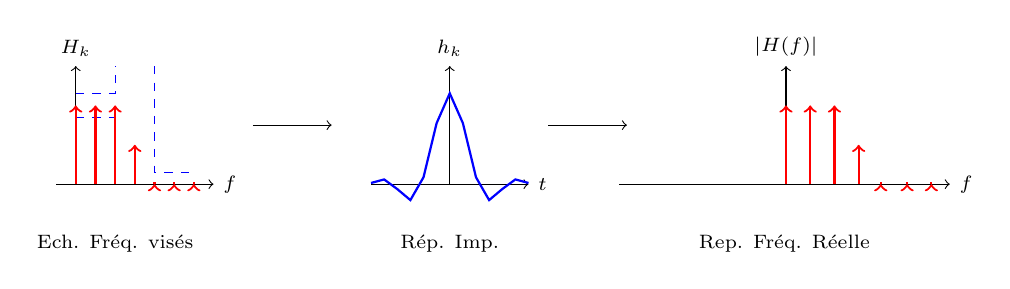
\begin{tikzpicture}
	\begin{scope}[scale=0.5]
	\draw[->] (-0.5,0)-- (3.5,0)node[right] {\scriptsize $f$} ;
%\draw (-0.3,-0.3) node {0};
\draw[->] (0,0)-- (0,3)node[above] {\scriptsize $H_k$};

\draw[dashed,blue](0,1.7)--(1,1.7)--(1,0);
\draw[dashed,blue](0,2.3)--(1,2.3)--(1,3);
\draw[dashed,blue](2,3)--(2,0.3)--(3,0.3);

	%\draw[thick,red]   (0,2)--(1.5,2)--(1.5,0)--(3,0);
	\draw[->,thick,red] (0,0)--(0,2);
	\draw[->,thick,red] (0.5,0)--(0.5,2);
	\draw[->,thick,red] (1,0)--(1,2);
		\draw[->,thick,red] (1.5,0)--(1.5,1);
	\draw[->,thick,red] (2,0)--(2,0);
	\draw[->,thick,red] (2.5,0)--(2.5,0);
	\draw[->,thick,red] (3,0)--(3,0);
	\draw[->] (4.5,1.5)--(6.5,1.5); 
	\draw (1,-1.5) node[text centered] {\scriptsize Ech. Fréq. visés};
	\end{scope}
	
	\begin{scope}[scale=0.5,xshift=9.5 cm]
	\draw[->] (-2,0)-- (2,0)node[right] {\scriptsize $t$} ;
\draw[->] (0,0)-- (0,3)node[above] {\scriptsize $h_k$};
\draw[thick,blue] plot coordinates{
(-6/3,0.006*5)
(-5/3,0.024*5)
(-4/3,-0.025*5)
(-3/3,-0.081*5)
(-2/3,0.035*5)
(-1/3,0.31*5)
(0/3,0.4615*5)
(1/3,0.31*5)
(2/3,0.035*5)
(3/3,-0.081*5)
(4/3,-0.025*5)
(5/3,0.024*5)
(6/3,0.006*5)};
\draw[->] (2.5,1.5)--(4.5,1.5); 
\draw (0,-1.5) node[text centered] {\scriptsize Rép. Imp.};
\end{scope}
	
	\begin{scope}[scale=1,xshift=9cm]
\draw[->] (-2.1,0)-- (2.1,0)node[right] {\scriptsize $f$} ;
\draw[->] (0.02,0)-- (0.02,1.5)node[above] {\scriptsize  $|H(f)|$};
\draw[thick,blue] plot file {module_freq_samp.txt};


\draw[->,thick,red] (0+0.02,0)--(0+0.02,1);
\draw[->,thick,red] (0.3077+0.02,0)--(0.3077+0.02,1);
\draw[->,thick,red] (0.6154+0.02,0)--(0.6154+0.02,1);
\draw[->,thick,red] (0.9231+0.02,0)--(0.9231+0.02,0.5);
\draw[->,thick,red] (1.2038+0.02,0)--(1.2038+0.02,0);
\draw[->,thick,red] (1.5385+0.02,0)--(1.5385+0.02,0);
\draw[->,thick,red] (1.8462+0.02,0)--(1.8462+0.02,0);
\draw (0,-0.75) node[text centered] {\scriptsize Rep. Fréq. Réelle};
\end{scope}
	
\end{tikzpicture}
\end{center}
\vspace{0.3cm}

\vspace{0.1cm}
\begin{enumerate}
\item<2-> On fixe des valeurs pour le spectre dans les trois régions
\item<3-> De ces valeurs on calcule la réponse impulsionnelle
\item<4-> Permet de réduire l'amplitude des oscillations dans une bande ou l'autre par rapport à la méthodes des fenêtres
\end{enumerate}


\end{frame}

\begin{frame} 
\frametitle{Méthode de l'échantillonnage en fréquence: Résumé}
\begin{center}
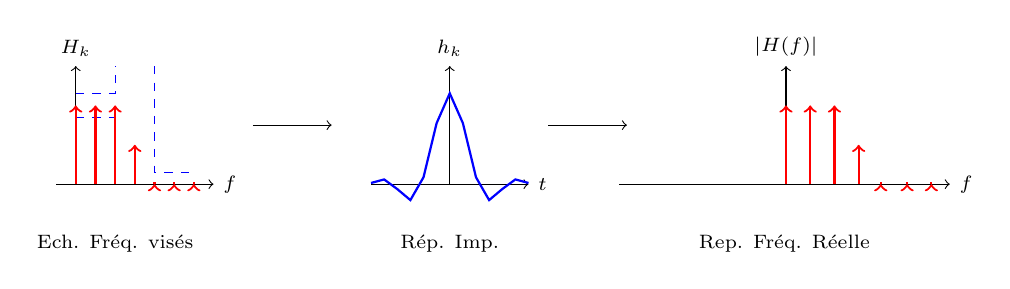
\begin{tikzpicture}
	\begin{scope}[scale=0.5]
	\draw[->] (-0.5,0)-- (3.5,0)node[right] {\scriptsize $f$} ;
%\draw (-0.3,-0.3) node {0};
\draw[->] (0,0)-- (0,3)node[above] {\scriptsize $H_k$};

\draw[dashed,blue](0,1.7)--(1,1.7)--(1,0);
\draw[dashed,blue](0,2.3)--(1,2.3)--(1,3);
\draw[dashed,blue](2,3)--(2,0.3)--(3,0.3);

	%\draw[thick,red]   (0,2)--(1.5,2)--(1.5,0)--(3,0);
	\draw[->,thick,red] (0,0)--(0,2);
	\draw[->,thick,red] (0.5,0)--(0.5,2);
	\draw[->,thick,red] (1,0)--(1,2);
		\draw[->,thick,red] (1.5,0)--(1.5,1);
	\draw[->,thick,red] (2,0)--(2,0);
	\draw[->,thick,red] (2.5,0)--(2.5,0);
	\draw[->,thick,red] (3,0)--(3,0);
	\draw[->] (4.5,1.5)--(6.5,1.5); 
	\draw (1,-1.5) node[text centered] {\scriptsize Ech. Fréq. visés};
	\end{scope}
	
	\begin{scope}[scale=0.5,xshift=9.5 cm]
	\draw[->] (-2,0)-- (2,0)node[right] {\scriptsize $t$} ;
\draw[->] (0,0)-- (0,3)node[above] {\scriptsize $h_k$};
\draw[thick,blue] plot coordinates{
(-6/3,0.006*5)
(-5/3,0.024*5)
(-4/3,-0.025*5)
(-3/3,-0.081*5)
(-2/3,0.035*5)
(-1/3,0.31*5)
(0/3,0.4615*5)
(1/3,0.31*5)
(2/3,0.035*5)
(3/3,-0.081*5)
(4/3,-0.025*5)
(5/3,0.024*5)
(6/3,0.006*5)};
\draw[->] (2.5,1.5)--(4.5,1.5); 
\draw (0,-1.5) node[text centered] {\scriptsize Rép. Imp.};
\end{scope}
	
	\begin{scope}[scale=1,xshift=9cm]
\draw[->] (-2.1,0)-- (2.1,0)node[right] {\scriptsize $f$} ;
\draw[->] (0.02,0)-- (0.02,1.5)node[above] {\scriptsize  $|H(f)|$};
\draw[thick,blue] plot file {module_freq_samp.txt};


\draw[->,thick,red] (0+0.02,0)--(0+0.02,1);
\draw[->,thick,red] (0.3077+0.02,0)--(0.3077+0.02,1);
\draw[->,thick,red] (0.6154+0.02,0)--(0.6154+0.02,1);
\draw[->,thick,red] (0.9231+0.02,0)--(0.9231+0.02,0.5);
\draw[->,thick,red] (1.2038+0.02,0)--(1.2038+0.02,0);
\draw[->,thick,red] (1.5385+0.02,0)--(1.5385+0.02,0);
\draw[->,thick,red] (1.8462+0.02,0)--(1.8462+0.02,0);
\draw (0,-0.75) node[text centered] {\scriptsize Rep. Fréq. Réelle};
\end{scope}
	
\end{tikzpicture}
\end{center}
\vspace{0.3cm}
Remarques:
\vspace{0.1cm}
\begin{itemize}
\item Méthode la plus "simple" 
\item Compromis largeur/ondulations
\item Performances similaires à la méthode des fenêtres
\end{itemize}


\end{frame}


\begin{frame}
\frametitle{Synthèse de filtres non-récursifs: Différentes méthodes}
Les méthodes suivent toute le même principe général :

\begin{center}
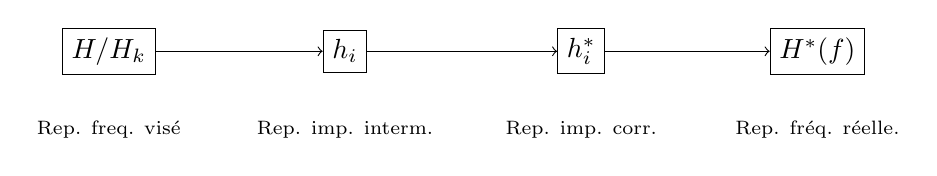
\begin{tikzpicture}
		\node[rectangle,draw,align=center] (I) at (1,0) {$H/H_k$};
		\draw (1,-1) node[text centered] {\scriptsize Rep. freq. visé};
		\node[rectangle,draw,align=center] (D) at (4,0) {$h_i$};
		\draw (4,-1) node[text centered] {\scriptsize Rep. imp. interm.};
		\node[rectangle,draw,align=center] (N) at (7,0) {$h_i^*$};
				\draw (7,-1) node[text centered] {\scriptsize Rep. imp. corr.};
		\node[rectangle,draw,align=center] (B) at (10,0) {$H^*(f)$};	
		\draw (10,-1) node[text centered]{\scriptsize Rep. fréq. réelle.};
		
		\draw[->] (I)--(D);
		\draw[->] (D)--(N);
		\draw[->] (N)--(B);
\end{tikzpicture}
\end{center}

Principales méthodes de synthèse de filtres non-récursifs:
\vspace{0.2cm}
\begin{itemize}
\item<2-> \textbf{Méthode des fenêtres} \only<7->{: Simple mais ondulation amplitude non-const. identique en bde passante et affablie}
\item<3-> \textbf{Méthode de l'échantillonnage en fréquence}\only<8->{ : Ondulation potentiellement réduite mais tjrs amplitude non-constante}
\item<4-> Méthode des moindres carrés  \only<9->{:idem}
\item<5-> Méthode itérative par TFD \only<10->{ : amplitude constante possible}
\item<6-> Méthode par approximation de
Tchebychev :\only<11->{spécification complète.
}
\end{itemize}

\end{frame}
\subsection{Synthèse de filtres récursifs}


\begin{frame}
\frametitle{Synthèse de filtres récursifs : Principe général}
Pour les filtres non-récursifs, on réglait les coeffs de la \textbf{réponse impulsionnelle}\\

\vspace{1 cm}
\only<2->{
Filtre récursif  $\rightarrow$ réponse impulsionnelle infinie...\\
}
\vspace{1 cm}
\only<3->{ 
\begin{block}{}
On travaille sur la \textbf{fonction de transfert} 
\end{block}
}

\end{frame}

\begin{frame}
\frametitle{Synthèse de filtres récursifs : Principe général}

\begin{block}{}
On travaille sur la \textbf{fonction de transfert} 
\end{block}

\vspace{1cm} 

Fonction de transfert en $z$ = \textbf{fonction continue }\\

\vspace{1cm}

\textbf{Comment représenter le filtre en numérique ? (nombre fini de termes)}


\end{frame}

\begin{frame}
\frametitle{Synthèse de filtres récursifs : Principe général}
\textbf{Comment représenter le filtre en numérique ? (nombre fini de termes)}\\
\vspace{1cm}
\only<1>{
\[\text{eq° différence  } \;\;\; y[n] = x[n] +  a y[n] \; \rightarrow  \; \frac{1}{1-a z^{-1}} \;\;\; \text{   fct° transfert} \]\\
}
\only<2->{
\[\text{eq° différence  } \;\;\; y[n] = x[n] + \mbox{\bfseries a} y[n] \; \rightarrow  \; \frac{1}{1-\mbox{\bfseries a} z^{-1}} \;\;\; \text{   fct° transfert} \]\\
}
\vspace{1cm} 

\only<3->{
\begin{block}{}
C'est le coefficient \bfseries{ a} qui est stocké par l'ordinateur (ou réglé dans les circuits
\end{block}
}



\end{frame}

\begin{frame}
\frametitle{Synthèse de filtres récursifs : Principe général}

 
\begin{block}{}
On travaille directement dans le \textbf{domaine fréquentiel.}
\end{block}
\vspace{1cm}
$\rightarrow$ On calcule les $a_k,b_k$ dans $H(z) = \frac{\displaystyle 1+ a_1 z + a_2 z^2 + \cdots + a_n z^n }{\displaystyle 1+ b_1 z + b_2 z^2 + \cdots + b_n z^n}$ \\
\vspace{1cm}

2 grandes classes de méthodes : 
\begin{itemize}
\item<2->  \only<2-3>{ Calcul direct des coefficients par fonctions modèles}
\only<4>{ \textbf{Calcul direct des coefficients par l'analogique}}
\vspace{0.3cm}

\item<3-> Techniques itératives

\end{itemize}
\end{frame}

\subsection{Synthèse de filtres récursifs: Calcul direct par l'analogique}

\begin{frame}
\frametitle{Synthèse de filtres récursifs: Calcul direct par l'analogique}
On s'inspire des filtres analogiques qu'on connait bien...\\
\vspace{1cm}
On part de $H(s)$ ... $\rightarrow$ Comment passer à $H(z)$ ?\\
\vspace{1cm}
\only<2->{
\begin{center} 
 $z = e^{sT_e}$ ? \only<3>{\textbf{NON.}}
\end{center}
} 
\end{frame}

\begin{frame}
\frametitle{Synthèse de filtres récursifs: Calcul direct par l'analogique}
$z = e^{sT_e}$ ne fonctionne pas... Pourquoi ?\\
\vspace{0.5cm}
\only<2->{
\textbf{Problème 1 }: Les fonctions de transferts doivent être des fractions rationnelles...\\
\vspace{0.5cm}
Or, si $H(s)$ est une fraction rationnelle $H(z = e^{sT_e})$ n'est pas une fraction rationnelle...\\
\vspace{0.5cm}
}

\only<3->{
\textbf{Problème 2} : Un système stable en analogique et converti de cette manière n'est pas forcément stable en numérique...\\

}

\only<4->{
\vspace{0.5cm}
\begin{block}{}
Nécessité de trouver une correspondance qui remplisse ces deux critères...
\end{block}
}

\end{frame}

\begin{frame}
\frametitle{Synthèse de filtres récursifs: Calcul direct par l'analogique}
\begin{center}
\begin{tikzpicture}
\draw[->](0,0)--(0,1) node[above]{$H(s)$};
\draw[->](0,0)--(1,0) node[right]{$s$};
\draw (0.5,-0.5) node[text centered]  {\scriptsize fct° transfert  analogique};


\draw[thick,blue] (0,0.8).. controls(0.9,0.8) and (0.25,0).. (0.9,0);

\only<2->{
\draw[->] (1.2,0.5)--(1.7,0.5);
\node[rectangle,draw,align=center] (I) at (3,0.5) {$z= f(s)$};
}

\only<3->{
\draw[->] (4.2,0.5)--(4.7,0.5);

\draw[->](5,0)--(5,1) node[above]{$H(z)$};
\draw[->](5,0)--(6,0) node[right]{$z$};

\draw[thick,red] (5,0.8).. controls(5.9,0.5) and (5.25,0.3).. (5.9,0);
\draw (5.5,-0.5) node[text centered]  { \scriptsize fct° transfert numérique};
}
\end{tikzpicture}
\end{center}
\vspace{0.3cm}

\begin{enumerate}
\item Choix d'une fonction analogique correspondant au gabarit
\vspace{0.2cm}
\item<2->  Choix d'une méthode de conversion pour passer de $s$ à $z$ 
\vspace{0.2cm}
\item<3-> Obtention d'une fonction de transfert en $z$ 
\end{enumerate}

\end{frame}

\begin{frame}
\frametitle{Synthèse de filtres récursifs: Calcul direct par l'analogique}
\begin{center}
\begin{tikzpicture}
\draw[->](0,0)--(0,1) node[above]{$H(s)$};
\draw[->](0,0)--(1,0) node[right]{$s$};
\draw (0.5,-0.5) node[text centered]  {\scriptsize fct° transfert  analogique};


\draw[thick,blue] (0,0.8).. controls(0.9,0.8) and (0.25,0).. (0.9,0);

\only<2->{
\draw[->] (1.2,0.5)--(1.7,0.5);
\node[rectangle,draw,align=center] (I) at (3,0.5) {$z= f(s)$};
}

\only<3->{
\draw[->] (4.2,0.5)--(4.7,0.5);

\draw[->](5,0)--(5,1) node[above]{$H(z)$};
\draw[->](5,0)--(6,0) node[right]{$z$};

\draw[thick,red] (5,0.8).. controls(5.9,0.5) and (5.25,0.3).. (5.9,0);
\draw (5.5,-0.5) node[text centered]  { \scriptsize fct° transfert numérique};
}
\end{tikzpicture}
\end{center}
\vspace{0.3cm}
\begin{itemize}
\item Approximation de la dérivée 
\item Invariance impulsionnelle
\item Transformation Bilinéaire
\end{itemize}

\end{frame}
\subsection{Approximation de la dérivée}

\begin{frame}
\frametitle{Synthèse de filtres récursifs: Approximation de la dérivée}
En analogique, \\
\vspace{0.2cm}
\[y(t) =  \frac{dx(t)}{dt}  \rightarrow  \; H(s) = s \]\\
\vspace{0.2cm} 
\only<2->{
En discret, on peut écrire:\\
\vspace{0.2cm}
\[y(t) = \frac{dy(t)}{dt} \; \;  \approx \; \;  y[n] = \frac{x[n]-x[n-1]}{T_e} \]\\
\vspace{0.2cm}
}
\only<3->{
\[  y[n] = \frac{x[n]-x[n-1]}{T_e} \; \rightarrow \;  H(z) = \frac{1 -z ^{-1}}{T_e} \]\\
\vspace{0.2cm}
}

\only<4->{
\[\boxed{s  \approx \frac{1-z^{-1}}{T_e}} \]
}
\end{frame}

\begin{frame}
\frametitle{Synthèse de filtres récursifs: Approximation de la dérivée}
Prenons le filtre passe-bas analogique suivant  :
\[ H(s) = \frac{1}{s+a} \; \;  \leftrightarrow \; \; \frac{dy(t)}{dt} + ay(t) = x(t) \]\\

\only<2->{
\vspace{0.5cm} 
\'Etude de la réponse en fréquence afin de pouvoir comparer
}

\only<3->{
\[H(s) = \frac{1}{s+a} \; \;  \rightarrow \; \; H(\nu) = \frac{1}{2j\pi \nu + a}\]
}
\end{frame}

\begin{frame}
\frametitle{Synthèse de filtres récursifs: Approximation de la dérivée}

\'Etude de la réponse en fréquence du passe-bas analogique afin de pouvoir comparer\\
\vspace{0.5cm}
\[H(s) = \frac{1}{s+a} \; \;  \rightarrow \; \; H(\nu) = \frac{1}{2j\pi \nu + a}\]\\
\vspace{0.5cm}

\begin{columns}
\column{60mm}
\only<2->{
\[ |H(j\omega)| = \frac{1}{\sqrt{\omega^2+a^2}} \]
}


\column{60mm}
\only<2->{
\[ \text{arg}(H(j\omega)) = -\arctan(\tan(\frac{\omega}{a})) \]
}


\end{columns}
\vspace{1cm}
\only<3->{
\textbf{On ne peut pas tracer sans avoir la valeur de $a$...}

}
\end{frame}

\begin{frame}
\frametitle{Synthèse de filtres récursifs: Approximation de la dérivée}
\[H(s) = \frac{1}{s+a} \; \;  \rightarrow \; \; H(\nu) = \frac{1}{2j\pi \nu + a}\]\\
\vspace{0.5 cm}
$a$ est homogène à... \only<2->{\textbf{une fréquence}} \\
\vspace{0.5 cm}
\only<3->{
Impact de $a$ sur le comportement du filtre ? \\
\vspace{0.3cm}
}

\only<4->{
\begin{columns}[T]
\column{60mm}
Si $\nu \rightarrow 0$,\\
\vspace{0.3cm}
\[H(\nu) = \frac{1}{2j\pi \nu + a} \rightarrow \frac{1}{a} \]

\column{60mm}
Si $\nu \rightarrow \infty$,\\
\vspace{0.3cm}
\[H(\nu) = \frac{1}{2j\pi \nu + a} \rightarrow \frac{1}{2j\pi \nu} \rightarrow 0 \]
\end{columns} 
}
\end{frame}

\begin{frame}
\frametitle{Synthèse de filtres récursifs: Approximation de la dérivée}
Impact de $a$ sur le comportement du filtre $H(\nu) = \frac{1}{2j\pi \nu + a}$\\
\vspace{0.2cm}
\begin{columns}[T]
\column{60mm}
Si $\nu \rightarrow 0$,\\
\vspace{0.2cm}
\[H(\nu) = \frac{1}{2j\pi \nu + a} \rightarrow \frac{1}{a} \]
\only<2->{
Si $a << 1$,\\
\[H(\nu) \rightarrow \frac{1}{a} \rightarrow H(\nu \rightarrow 0) >> 1 \]\\
\vspace{0.2cm}
Si $a >> 1$,\\
\[H(\nu)  \rightarrow \frac{1}{a} \rightarrow H(\nu \rightarrow 0) << 1 \]
}

\column{60mm}
Si $\nu \rightarrow \infty$,\\
\vspace{0.2cm}
\[H(\nu)  \rightarrow \frac{1}{2j\pi \nu} \rightarrow 0 \]\\
\vspace{1cm}
\only<3->{
plus $a$ est grand, plus $H(\nu)$ ira lentement vers 0
}
\end{columns} 



\end{frame}

\begin{frame}
\frametitle{Synthèse de filtres récursifs: Approximation de la dérivée}

On peut donc tracer la réponse pour différents régimes (suivant $a$)\\
\vspace{0.5cm}
\[H(s) = \frac{1}{s+a} \; \;  \rightarrow \; \; H(\nu) = \frac{1}{2j\pi \nu + a}\]\\
\vspace{0.5cm}

\begin{columns}
\column{60mm}

\only<2->{
\begin{center}
\begin{tikzpicture}
\begin{scope}[scale=2] 
\draw[->] (0,0)--(2,0) node[right] { $\scriptstyle \nu$};
\draw[->] (0,0) -- (0,1.5) node[above] {$\scriptstyle |H(\nu)|$} ;

%\draw (0.5,-0.4) node {$\frac{f_e}{2}$};

\draw[domain=0.065:1.9,color=blue!50!cyan,samples=30] plot (\x,{1/sqrt((10*\x)^2 + 0.1^2))});
\draw[domain=0:1.9,color=blue,samples=30] plot (\x,{1/sqrt((10*\x)^2 + 2^2))});

\draw[color=blue!50!cyan] (1.2,1.25)--(1.4,1.25) node[right,color=black] {\scriptsize $a<<1$};
\draw[color=blue] (1.2,1)--(1.4,1) node[right,color=black] {\scriptsize $a>>1$};
\end{scope}
\end{tikzpicture}
\end{center}
}

\column{60mm}

\only<2->{
\begin{center}
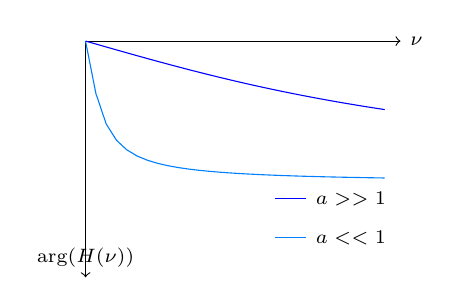
\begin{tikzpicture}
\begin{scope}[scale=2] 
\draw[->] (0,0)--(2,0) node[right] { $\scriptstyle \nu$};
\draw[->] (0,0) -- (0,-1.5) node[above] {$\scriptstyle \text{arg}(H(\nu))$} ;

%\draw (0.5,-0.4) node {$\frac{f_e}{2}$};

\draw[domain=0.0:1.9,color=blue!50!cyan,samples=30] plot (\x,{-0.01*atan(\x/0.1)});
\draw[domain=0.0:1.9,color=blue,samples=30] plot (\x,{-0.01*atan(\x/2)});

\draw[color=blue!50!cyan] (1.2,-1.25)--(1.4,-1.25) node[right,color=black] {\scriptsize $a<<1$};
\draw[color=blue] (1.2,-1)--(1.4,-1) node[right,color=black] {\scriptsize $a>>1$};
\end{scope}
\end{tikzpicture}
\end{center}
}

%\draw[->] (-1,0)--(1,0) node[right] { $\scriptstyle \omega$};
%\draw[->] (0,-1)-- (0,1) node[above] {$\scriptstyle |H(\omega)|$}; 
%
%\draw[domain= 0.5:1,color=blue,samples=30] plot (\x,{\x-1});
%\draw[domain=-0.5:0.5,color=blue,samples=30] plot (\x,{\x});
%\draw[domain= -1:-0.5,color=blue,samples=30] %\end{tikzpicture}
%\end{center}


\end{columns}

\end{frame}



\begin{frame}
\frametitle{Synthèse de filtres récursifs: Approximation de la dérivée}
Maintenant on passe en $z$
\vspace{0.5cm}
\[H(s) = \frac{1}{s+a} \; \;  \rightarrow \; \; H(z) = \frac{1}{\frac{1-z^{-1}}{T_e}+ a} = \frac{T_e}{1-z^{-1}+ a T_e}\]\\
\only<2->{
\vspace{0.5cm} 
On passe en fréquence, 
\[H(z) = \frac{T_e}{1-z^{-1}+ a T_e} \rightarrow H(\nu) = \frac{T_e}{1-e^{-j2\pi \nu T_e}+ a T_e}\]

}

\end{frame}

\begin{frame} 
\frametitle{Synthèse de filtres récursifs: Approximation de la dérivée}
Réponse en fréquence du filtre en $z$\\
\vspace{0.1cm}
\[H(\nu) =  \frac{T_e}{1-e^{-j2\pi \nu T_e}+ a T_e}\]\\
\vspace{0.2cm}
\only<2->{
En discret, $\nu \in [0,\nu_e/2]$\\
\vspace{0.2cm}
}
\only<3->{
\begin{columns}
\column{20mm}
\[H(0) = \frac{T_e}{a T_e} \]
\column{50mm}
\[H(\nu_e/4) = \frac{T_e}{1- j +a T_e} \]
\column{30mm}
\[H(\nu_e/2) = \frac{T_e}{2 + a T_e} \]
\end{columns}

}

\only<4->{
\begin{columns}
\column{20mm}
\[|H(0)| = \frac{T_e}{a T_e} \]
\column{50mm}
\[|H(\nu_e/4)| = \frac{T_e}{\sqrt{(1 + aT_e)^2 + 1}} \]
\column{30mm}
\[|H(\nu_e/2)| = \frac{T_e}{2 + a T_e} \]
\end{columns}

}

\only<5->{
\vspace{0.2cm}
Comme précédemment, on va avoir $a>> T_e$ et $a<<T_e$
}

\end{frame}

\begin{frame}
\frametitle{Synthèse de filtres récursifs: Approximation de la dérivée}
Réponse en fréquence du filtre en $z$\\
\vspace{0.1cm}
\[H(\nu) =  \frac{T_e}{1-e^{-j2\pi \nu T_e}+ a T_e}\]\\


\begin{columns}
\column{60mm}

\only<2->{
\begin{center}
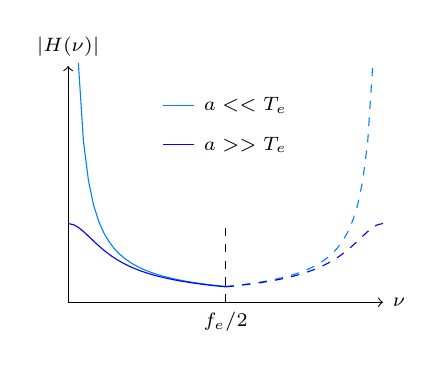
\begin{tikzpicture}
\begin{scope}[scale=2] 
\draw[->] (0,0)--(2,0) node[right] { $\scriptstyle \nu$};
\draw[->] (0,0) -- (0,1.5) node[above] {$\scriptstyle |H(\nu)|$} ;

%\draw (0.5,-0.4) node {$\frac{f_e}{2}$};

\draw[domain=0.065:1,color=blue!50!cyan,samples=30] plot (\x,{1/sqrt((10*\x)^2 + 0.1^2))});
\draw[domain=0:1,color=blue,samples=30] plot (\x,{1/sqrt((10*\x)^2 + 2^2))});

\begin{scope}[xshift=2cm]
\draw[dashed,domain=-1:-0.065,color=blue!50!cyan,samples=30] plot (\x,{1/sqrt((10*\x)^2 + 0.1^2))});
\draw[dashed,domain=-1:0,color=blue,samples=30] plot (\x,{1/sqrt((10*\x)^2 + 2^2))});
\end{scope}

\draw[color=blue!50!cyan] (0.6,1.25)--(0.8,1.25) node[right,color=black] {\scriptsize $a<<T_e$};
\draw[color=blue] (0.6,1)--(0.8,1) node[right,color=black] {\scriptsize $a>>T_e$};
\draw[dashed] (1,0)node[below] {\scriptsize $f_e/2$}--(1,0.5);
\end{scope}


\end{tikzpicture}
\end{center}
}

\column{60mm}

\only<2->{
\begin{center}
\begin{tikzpicture}
\begin{scope}[scale=2] 
\draw[->] (0,0)--(2,0) node[right] { $\scriptstyle \nu$};
\draw[->] (0,-0.8)  -- (0,0.8) node[above] {$\scriptstyle \text{arg}(H(\nu))$}  ;

%\draw (0.5,-0.4) node {$\frac{f_e}{2}$};
%
%\draw[domain=0.1:1.9,color=blue!50!cyan,samples=30] plot (\x,{-0.1*sin(\x/(2*pi))});
%\draw[domain=-1:1,color=blue,samples=50] plot (\x,{sin(acos((\x))});
%\begin{scope}[xshift=1cm]
\draw[dashed,domain=0:2,color=blue!50!cyan,samples=30] plot (\x,{-0.01*atan(-sin(3.14*\x r)/(1-cos(3.14*\x r)+0.1))});
\draw[dashed,domain=0:2,color=blue,samples=30] plot (\x,{-0.01*atan(-sin(3.14*\x r)/(1-cos(3.14*\x r)+10))});
\draw[domain=0:1,color=blue!50!cyan,samples=30] plot (\x,{-0.01*atan(-sin(3.14*\x r)/(1-cos(3.14*\x r)+0.1))});
\draw[domain=0:1,color=blue,samples=30] plot (\x,{-0.01*atan(-sin(3.14*\x r)/(1-cos(3.14*\x r)+10))});
%\end{scope}

\draw[color=blue!50!cyan] (1.2,-1.25)--(1.4,-1.25) node[right,color=black] {\scriptsize $a<<1$};
\draw[color=blue] (1.2,-1)--(1.4,-1) node[right,color=black] {\scriptsize $a>>1$};
\draw[dashed] (1,-0.5)node[below] {\scriptsize $f_e/2$}--(1,0);
\end{scope}
\end{tikzpicture}
\end{center}
}


\end{columns}

\end{frame}

\begin{frame} 
\frametitle{Synthèse de filtres récursifs: Approximation de la dérivée}
On peut maintenant comparer le continu et le discret:\\ 
\vspace{0.3cm}
\begin{columns}
\column{60mm}
continu $\nu \in [0,\infty]$:
\[H(\nu) = \frac{1}{2j\pi \nu + a}\]
\vspace{0.1cm}
\begin{center}
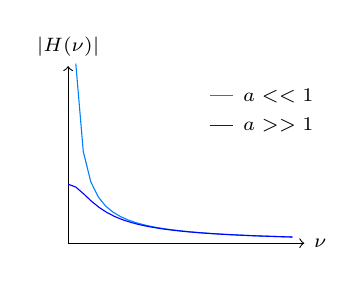
\begin{tikzpicture}
\begin{scope}[scale=1.5] 
\draw[->] (0,0)--(2,0) node[right] { $\scriptstyle \nu$};
\draw[->] (0,0) -- (0,1.5) node[above] {$\scriptstyle |H(\nu)|$} ;

%\draw (0.5,-0.4) node {$\frac{f_e}{2}$};

\draw[domain=0.065:1.9,color=blue!50!cyan,samples=30] plot (\x,{1/sqrt((10*\x)^2 + 0.1^2))});
\draw[domain=0:1.9,color=blue,samples=30] plot (\x,{1/sqrt((10*\x)^2 + 2^2))});

\draw[color=blue!50!cyan] (1.2,1.25)--(1.4,1.25) node[right,color=black] {\scriptsize $a<<1$};
\draw[color=blue] (1.2,1)--(1.4,1) node[right,color=black] {\scriptsize $a>>1$};
\end{scope}
\end{tikzpicture}
\end{center}

\column{60mm}
discret $\nu \in [0,\nu_e/2]$:
\[H(\nu) = \frac{T_e}{1-e^{-j2\pi \nu T_e}+ a T_e}\]
\vspace{0.1cm}
\begin{center}
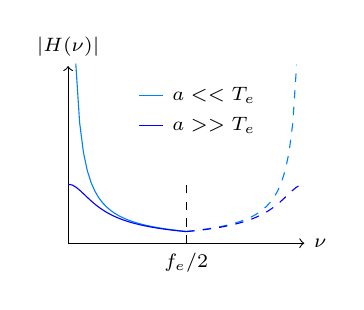
\begin{tikzpicture}
\begin{scope}[scale=1.5] 
\draw[->] (0,0)--(2,0) node[right] { $\scriptstyle \nu$};
\draw[->] (0,0) -- (0,1.5) node[above] {$\scriptstyle |H(\nu)|$} ;

%\draw (0.5,-0.4) node {$\frac{f_e}{2}$};

\draw[domain=0.065:1,color=blue!50!cyan,samples=30] plot (\x,{1/sqrt((10*\x)^2 + 0.1^2))});
\draw[domain=0:1,color=blue,samples=30] plot (\x,{1/sqrt((10*\x)^2 + 2^2))});

\begin{scope}[xshift=2cm]
\draw[dashed,domain=-1:-0.065,color=blue!50!cyan,samples=30] plot (\x,{1/sqrt((10*\x)^2 + 0.1^2))});
\draw[dashed,domain=-1:0,color=blue,samples=30] plot (\x,{1/sqrt((10*\x)^2 + 2^2))});
\end{scope}

\draw[color=blue!50!cyan] (0.6,1.25)--(0.8,1.25) node[right,color=black] {\scriptsize $a<<T_e$};
\draw[color=blue] (0.6,1)--(0.8,1) node[right,color=black] {\scriptsize $a>>T_e$};
\draw[dashed] (1,0)node[below] {\scriptsize $f_e/2$}--(1,0.5);
\end{scope}


\end{tikzpicture}
\end{center}

\end{columns}
\begin{itemize}
\item On perd les caractéristiques du filtres au delà de $f_e/2$
\end{itemize}

\end{frame}

\begin{frame}
\frametitle{Synthèse de filtres récursifs: Approximation de la dérivée}
Resumé:
\only<2->{
\[ y(t) = \frac{dy(t)}{dt} \; \;  \approx \; \;  y[n] = \frac{x[n]-x[n-1]}{T_e} \rightarrow \boxed{s  \approx \frac{1-z^{-1}}{T_e}} \]
\vspace{0.1cm}
}
\only<3->{
\[H(s) = \frac{1}{s+a} \; \;  \rightarrow \; \; H(z) = \frac{1}{\frac{1-z^{-1}}{T_e}+ a} = \frac{T_e}{1-z^{-1}+ a T_e}\]
}

\only<4->{
\begin{columns}
\column{60mm}
\vspace{0.1cm}
\begin{center}
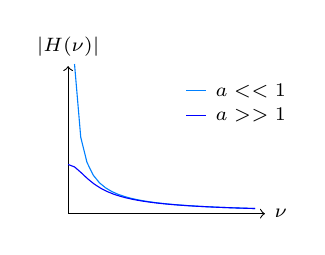
\begin{tikzpicture}
\begin{scope}[scale=1.25] 
\draw[->] (0,0)--(2,0) node[right] { $\scriptstyle \nu$};
\draw[->] (0,0) -- (0,1.5) node[above] {$\scriptstyle |H(\nu)|$} ;

%\draw (0.5,-0.4) node {$\frac{f_e}{2}$};

\draw[domain=0.065:1.9,color=blue!50!cyan,samples=30] plot (\x,{1/sqrt((10*\x)^2 + 0.1^2))});
\draw[domain=0:1.9,color=blue,samples=30] plot (\x,{1/sqrt((10*\x)^2 + 2^2))});

\draw[color=blue!50!cyan] (1.2,1.25)--(1.4,1.25) node[right,color=black] {\scriptsize $a<<1$};
\draw[color=blue] (1.2,1)--(1.4,1) node[right,color=black] {\scriptsize $a>>1$};
\end{scope}
\end{tikzpicture}
\end{center}

\column{60mm}
\vspace{0.1cm}
\begin{center}
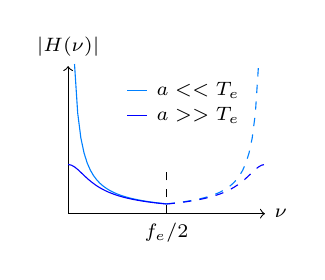
\begin{tikzpicture}
\begin{scope}[scale=1.25] 
\draw[->] (0,0)--(2,0) node[right] { $\scriptstyle \nu$};
\draw[->] (0,0) -- (0,1.5) node[above] {$\scriptstyle |H(\nu)|$} ;

%\draw (0.5,-0.4) node {$\frac{f_e}{2}$};

\draw[domain=0.065:1,color=blue!50!cyan,samples=30] plot (\x,{1/sqrt((10*\x)^2 + 0.1^2))});
\draw[domain=0:1,color=blue,samples=30] plot (\x,{1/sqrt((10*\x)^2 + 2^2))});

\begin{scope}[xshift=2cm]
\draw[dashed,domain=-1:-0.065,color=blue!50!cyan,samples=30] plot (\x,{1/sqrt((10*\x)^2 + 0.1^2))});
\draw[dashed,domain=-1:0,color=blue,samples=30] plot (\x,{1/sqrt((10*\x)^2 + 2^2))});
\end{scope}

\draw[color=blue!50!cyan] (0.6,1.25)--(0.8,1.25) node[right,color=black] {\scriptsize $a<<T_e$};
\draw[color=blue] (0.6,1)--(0.8,1) node[right,color=black] {\scriptsize $a>>T_e$};
\draw[dashed] (1,0)node[below] {\scriptsize $f_e/2$}--(1,0.5);
\end{scope}


\end{tikzpicture}
\end{center}

\end{columns}

}

\end{frame}

\begin{frame}
\frametitle{Synthèse de filtres récursifs: Approximation de la dérivée}
Remarques:\\
\vspace{0.1cm}
\begin{itemize}
\item On a approximé la dérivée d'un certaine manière mais d'autres formules plus complexes sont possibles...
\item Possiblement difficile de synthétiser des filtres passe-haut.. 
\end{itemize}
\label{rajouter passe haut si le temps le permet}
\end{frame}

\subsection{Invariance impulsionnelle}
\begin{frame}
\frametitle{Invariance impulsionnelle}
Approche plus "directe"\\
\vspace{0.1cm}
\only<2->{
\begin{center}
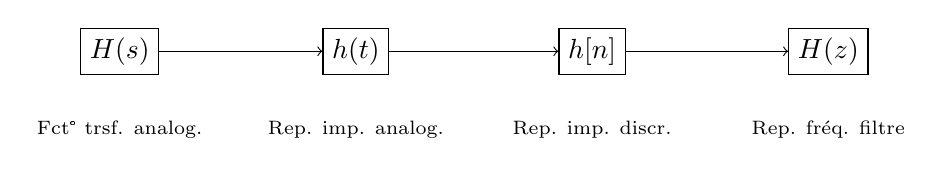
\begin{tikzpicture}
		\node[rectangle,draw,align=center] (I) at (1,0) {$H(s)$};
		\draw (1,-1) node[text centered] {\scriptsize Fct° trsf. analog.};
		\node[rectangle,draw,align=center] (D) at (4,0) {$h(t)$};
		\draw (4,-1) node[text centered] {\scriptsize Rep. imp. analog.};
		\node[rectangle,draw,align=center] (N) at (7,0) {$h[n]$};
				\draw (7,-1) node[text centered] {\scriptsize Rep. imp. discr.};
		\node[rectangle,draw,align=center] (B) at (10,0) {$H(z)$};	
		\draw (10,-1) node[text centered]{\scriptsize Rep. fréq. filtre};
		\draw[->] (I)--(D);
		\draw[->] (D)--(N);
		\draw[->] (N)--(B);
\end{tikzpicture}
\end{center}
}
\begin{enumerate}
\item<3-> On part d'une fonction analogique avec les bonnes propriétés (passe-bas, passe-haut, etc...)
\item<4-> On calcule sa réponse impulsionnelle en temporel
\item<5-> On échantillonne cette réponse impulsionnelle 
\item<6-> On prend la transformée en $z$ de cette réponse impulsionnelle échantillonnée pour obtenir la fonction de transfert
\end{enumerate}
\end{frame}

\begin{frame}
\frametitle{Invariance impulsionnelle}
\begin{center}
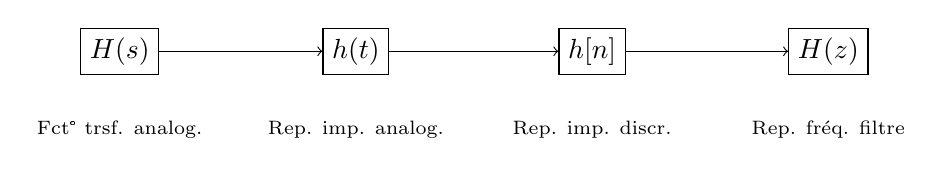
\begin{tikzpicture}
		\node[rectangle,draw,align=center] (I) at (1,0) {$H(s)$};
		\draw (1,-1) node[text centered] {\scriptsize Fct° trsf. analog.};
		\node[rectangle,draw,align=center] (D) at (4,0) {$h(t)$};
		\draw (4,-1) node[text centered] {\scriptsize Rep. imp. analog.};
		\node[rectangle,draw,align=center] (N) at (7,0) {$h[n]$};
				\draw (7,-1) node[text centered] {\scriptsize Rep. imp. discr.};
		\node[rectangle,draw,align=center] (B) at (10,0) {$H(z)$};	
		\draw (10,-1) node[text centered]{\scriptsize Rep. fréq. filtre};
		\draw[->] (I)--(D);
		\draw[->] (D)--(N);
		\draw[->] (N)--(B);
\end{tikzpicture}
\end{center}
\vspace{0.3cm}
MAIS...
\begin{itemize}
\item<2-> Filtre récursif $\rightarrow$ réponse impulsionnelle infinie...
\vspace{0.2cm}
\item<3-> Filtre numérique $\rightarrow$  représentation à l'aide d'un nombre fini de termes...
\item<4-> \textbf{Comment faire la conversion en pratique ?...}
\end{itemize}

\end{frame}

\begin{frame} 
\frametitle{Invariance impulsionelle}
Dans les faits, passage direct
\begin{center}
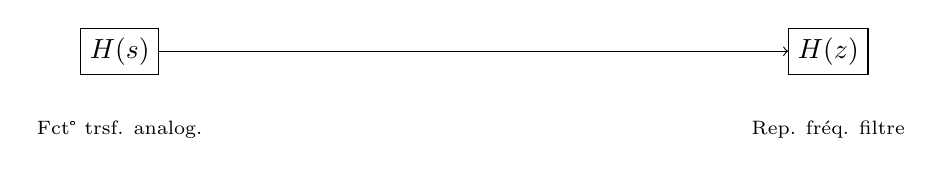
\begin{tikzpicture}
		\node[rectangle,draw,align=center] (I) at (1,0) {$H(s)$};
		\draw (1,-1) node[text centered] {\scriptsize Fct° trsf. analog.};

		\node[rectangle,draw,align=center] (B) at (10,0) {$H(z)$};	
		\draw (10,-1) node[text centered]{\scriptsize Rep. fréq. filtre};
		\draw[->] (I)--(B);
\end{tikzpicture}
\end{center}
\vspace{0.2cm}
\only<2->{
\underline{Rappel}: Synthétiser un filtre récursif = déterminer les coeff dans la fonction de transfert 
}
\vspace{0.2cm}
\only<3->{
\begin{block}{}
Principe: établir une correspondance mathématique entre les coefficients en analogique et les coefficients en numérique
\end{block}
}
\end{frame}

\begin{frame}
\frametitle{Invariance impulsionnelle}
Chose importante:  Soit une fonction de transfert $H(s)$, et deux entiers $m,n$ tels que $m < n$
\vspace{0.2cm}
\[ H(s)  = \frac{1+ a_1 s + a_2 s^2 + \cdots + a_n s^m }{1+ b_1 s + b_2 s^2 + \cdots + b_n s^n} =  \frac{(s-z_1)(s-z_2)...(s-z_n)}{(s-p_1)(s-p_2)...(s-p_n)}\] 
\vspace{0.2cm}
zéros : ensemble des $z_n$ \hspace{2 cm}  pôles : ensemble des $p_n$
\vspace{0.2cm}
\only<2->{
Il est possible de décomposer $H(s)$ en éléments simples\\
\vspace{0.1cm}
\[ H(s)  =  \frac{(s-z_1)(s-z_2)...(s-z_n)}{(s-p_1)(s-p_2)...(s-p_n)} = \frac{c_1}{s-p_1} + \frac{c_2}{s-p_2} + \cdots + \frac{c_n}{s-p_n} \] 
}

\only<3->{
\underline{Important }: les pôles $p_n$ ne changent pas de valeur entre les deux représentations
}
\end{frame}

\begin{frame}
\frametitle{Invariance impulsionnelle}
Pour un filtre récursif analogique, on peut donc écrire en général 
\[ H(s)  =  \frac{(s-z_1)(s-z_2)...(s-z_n)}{(s-p_1)(s-p_2)...(s-p_n)} = \frac{c_1}{s-p_1} + \frac{c_2}{s-p_2} + \cdots + \frac{c_n}{s-p_n} \] \\
\vspace{0.2cm}
Un filtre récursif quelconque peut donc s'écrire comme une somme de filtres passe-bas:\\
\vspace{0.2cm}
\[ H(s)  = \frac{c_1}{s-p_1} + \frac{c_2}{s-p_2} + \cdots + \frac{c_n}{s-p_n} = H_1(s) + H_2(s) + \cdots  + H_n(z)\]

\end{frame}

\begin{frame}
\frametitle{Invariance impulsionnelle} 
Pour un filtre passe bas avec un pôle $p_k$,\\
\vspace{0.1cm}
\[ H_k(s) = \frac{c_k}{s-p_k} \rightarrow h_k(t) = c_k e^{p_k t} \]\\
\vspace{0.1cm}
\only<2->{
On peut alors appliquer le principe d'invariance impulsionnelle et échantillonner la réponse impulsionnelle\\
\vspace{0.1cm}
\[h_k(t) = c_k e^{p_k t} \rightarrow  h_k[n] = c_k e^{p_k n T_e} \]\\
}
\only>3->{
\vspace{0.1cm}
On prend alors la transformée en $z$ de $h_k[n]$
\vspace{0.1cm}
\[ h_k[n] = c_k e^{p_k n T_e} \rightarrow H_k(z)= \frac{c_k}{1-e^{p_k T_e}z^{-1}}\]
}
\end{frame}


\begin{frame}
\frametitle{Invariance impulsionnelle} 
Donc \\
\vspace{0.1cm}
\[ H(s)  =  \frac{1+ a_1 s + a_2 s^2 + \cdots + a_n s^m }{1+ b_1 s + b_2 s^2 + \cdots + b_n s^n} = \frac{c_1}{s-p_1} + \frac{c_2}{s-p_2} + \cdots + \frac{c_n}{s-p_n} \]\\
\vspace{0.1cm}
\only<2->{
et,
\[ H_k(s) = \frac{c_k}{s-p_k} \rightarrow H_k(z)= \frac{c_k}{1-e^{p_k T_e}z^{-1}}\]
}
\only<3->{
\[ H(s) = \frac{1+ a_1 s + a_2 s^2 + \cdots + a_n s^m }{1+ b_1 s + b_2 s^2 + \cdots + b_n s^n}  \] 

\[ \rightarrow H(z) = \frac{c_1}{1-e^{p_1 T_e}z^{-1}} + \frac{c_2}{1-e^{p_2 T_e}z^{-1}}  + \cdots + \frac{c_n}{1-e^{p_n T_e}z^{-1}} \]
}
\end{frame}

\begin{frame}
\frametitle{Invariance impulsionnelle: Résumé} 
Pour résumer: \\
\begin{center}
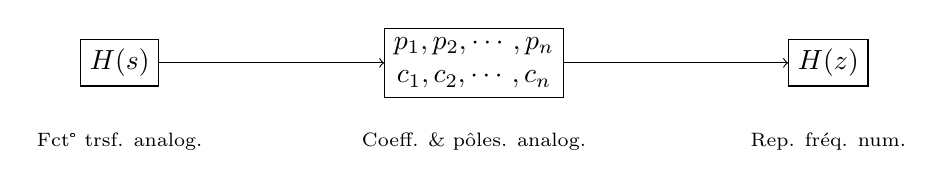
\begin{tikzpicture}
		\node[rectangle,draw,align=center] (I) at (1,0) {$H(s)$};
		\draw (1,-1) node[text centered] {\scriptsize Fct° trsf. analog.};
		\node[rectangle,draw,align=center] (D) at (5.5,0) {$p_1, p_2, \cdots, p_n$\\  $c_1, c_2, \cdots, c_n$};
		\draw (5.5,-1) node[text centered] {\scriptsize Coeff. \& pôles. analog.};
		\node[rectangle,draw,align=center] (B) at (10,0) {$H(z)$};	
		\draw (10,-1) node[text centered]{\scriptsize Rep. fréq. num.};
		\draw[->] (I)--(D);
		\draw[->] (D)--(B);
\end{tikzpicture}
\end{center}
\vspace{0.1cm}
\begin{enumerate}
\item<2-> On choisit un filtre $H(s)$ analogique
\vspace{0.5cm} 
\item<3-> On calcule sa décomposition en éléments simple pour obtenir les pôles $p_1, p_2, \cdots, p_n$ et les constantes $c_1, c_2, \cdots, c_n$ 
\vspace{0.5cm} 
\item<4-> On calcule $H(z)$ en sommant les fonctions  $\frac{\displaystyle c_k}{ \displaystyle 1-e^{p_k T_e}z^{-1}}$
\end{enumerate}
\end{frame}

\begin{frame}
\frametitle{Invariance impulsionnelle: Remarques} 

\begin{center}
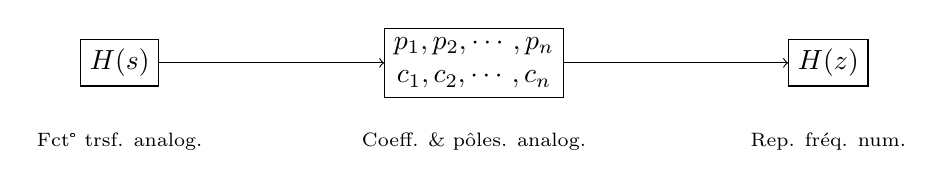
\begin{tikzpicture}
		\node[rectangle,draw,align=center] (I) at (1,0) {$H(s)$};
		\draw (1,-1) node[text centered] {\scriptsize Fct° trsf. analog.};
		\node[rectangle,draw,align=center] (D) at (5.5,0) {$p_1, p_2, \cdots, p_n$\\  $c_1, c_2, \cdots, c_n$};
		\draw (5.5,-1) node[text centered] {\scriptsize Coeff. \& pôles. analog.};
		\node[rectangle,draw,align=center] (B) at (10,0) {$H(z)$};	
		\draw (10,-1) node[text centered]{\scriptsize Rep. fréq. num.};
		\draw[->] (I)--(D);
		\draw[->] (D)--(B);
\end{tikzpicture}
\end{center}
\vspace{0.1cm}
Remarques :
\vspace{0.1cm}
\begin{itemize}
\item<2-> Méthode utilisée dans certains calculateurs pour simuler des systèmes analogiques
\vspace{0.3cm} 
\item<3-> Comme dans la méthode précedente, le repliment spectral due à l'échantillonnage  rend compliquée la conversion des filtres passe-haut sans fréquence d'échantillonnage importante...

\end{itemize}
\end{frame}

\subsection{Transformation Bilinéaire}
\begin{frame}
\frametitle{Synthèse de filtres récursifs:Transformation Bilinéaire} 
Synthèse de filtre récursifs par le biais de filtres analogiques :  $H(s) \rightarrow H(z)$\\
Propriétés requises : \\
\begin{itemize}
\item<2-> fraction rationnelle en $s$ $\rightarrow$ fraction rationnelle en $z$
\vspace{0.5cm}
\item<3-> filtre stable en  $s$ $\rightarrow$ filtre stable en  $z$
\vspace{0.5cm}
\item<4-> Conservation des propriétés en amplitude (ex: passe-haut $\rightarrow$ passe-haut)
\end{itemize}
\only<5->{
\vspace{0.4cm}
Bon compromis : \textbf{Transformation bilinéaire}
}
\end{frame}

\begin{frame}
\frametitle{Synthèse de filtres récursifs:Transformation Bilinéaire} 
Transformation bilinéaire : 
\[ s = \frac{2}{T_e} \frac{1-z^{-1}}{1+z^{-1}} \] \\
\vspace{0.2cm}
\only<2->{
On peut le comprendre ainsi : \\
\vspace{0.1cm}
\[ z = e^{sT_e} =  \frac{e^{s\frac{T_e}{2}}}{e^{-s\frac{T_e}{2}}} \approx \frac{1 + s \frac{T_e}{2}}{1 - s \frac{T_e}{2}}  \]

}
\end{frame}

\begin{frame}
\frametitle{Synthèse de filtres récursifs:Transformation Bilinéaire}
Appliquons la transformation bilinéaire au filtre étudié précédemment:
\[ H(s) = \frac{1}{s+a} \]\\
\vspace{0.2cm}
\only<3->{
\[  H(s) = \frac{1}{s+a} \rightarrow H(z) = \frac{1}{\frac{2}{T_e} \frac{1-z^{-1}}{1+z^{-1}}+a} =\frac{T_e(1+z^{-1})}{2(1-z^{-1}) + aT_e(1+z^{-1})} \]
}
\vspace{0.2cm}
\only<4->{
Etudions la réponse en fréquence du filtre numérique...
}
\end{frame}

\begin{frame}
\frametitle{Synthèse de filtres récursifs:Transformation Bilinéaire}
Réponse en fréquence :
\vspace{0.2cm}
\[ H(z)  =\frac{T_e(1+z^{-1})}{2(1-z^{-1}) + aT_e(1+z^{-1})}\]
 \vspace{0.2cm}
 \only<2->{
\[ \rightarrow H(\nu) =  \frac{T_e(1+e^{-j2 \pi \nu T_e})}{2(1-e^{-j2 \pi \nu T_e}) + aT_e(1+e^{-j2 \pi \nu T_e})}\]
\vspace{0.2cm}
}
 \only<3->{
\[ \rightarrow H(\nu) =  \frac{jT_e\; \cos(\pi \nu T_e)}{2\sin(\pi \nu T_e)+ ajT_e\; \cos(\pi \nu T_e)}\]
}
\end{frame}


\begin{frame}
\frametitle{Synthèse de filtres récursifs:Transformation Bilinéaire}
Réponse en fréquence :  Amplitude
\vspace{0.2cm}
\[H(\nu) =  \frac{jT_e\; \cos(\pi \nu T_e)}{2\sin(\pi \nu T_e)+ ajT_e\; \cos(\pi \nu T_e)}\]
\vspace{0.2cm}
\[|H(\nu)| =  \frac{|jT_e\; \cos(\pi \nu T_e)|}{|2\sin(\pi \nu T_e)+ ajT_e\; \cos(\pi \nu T_e)|}\]
\vspace{0.2cm}
\[|H(\nu)| =  \frac{|T_e\; \cos(\pi \nu T_e)|}{\sqrt{4\sin^2(\pi \nu T_e)+ a^2T_e^2\; \cos^2(\pi \nu T_e)}}\]

\end{frame}

\begin{frame}
\frametitle{Synthèse de filtres récursifs:Transformation Bilinéaire}
\vspace{0.2cm}
\[|H(\nu)| =  \frac{|T_e\; \cos(\pi \nu T_e)|}{\sqrt{4\sin^2(\pi \nu T_e)+ a^2T_e^2\; \cos^2(\pi \nu T_e)}}\]

\begin{center}
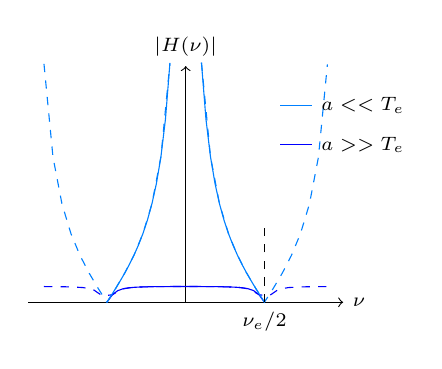
\begin{tikzpicture}
\begin{scope}[scale=2] 
\draw[->] (-1,0)--(1,0) node[right] { $\scriptstyle \nu$};
\draw[->] (0,0) -- (0,1.5) node[above] {$\scriptstyle |H(\nu)|$} ;

%\draw (0.5,-0.4) node {$\frac{f_e}{2}$};

\draw[dashed,domain=-0.9:0.9,color=blue,samples=30] plot (\x,{abs(cos(3.14*\x r))/(sqrt((2*sin(3.14 *\x r))^2 + (10*cos(3.14*\x r))^2))});
\draw[domain=-0.5:0.5,color=blue,samples=30] plot (\x,{abs(cos(3.14*\x r))/(sqrt((2*sin(3.14 *\x r))^2 + (10*cos(3.14*\x r))^2))});
\draw[dashed,domain=-0.9:-0.1,color=blue!50!cyan,samples=15] plot (\x,{abs(cos(3.14*\x r))/sqrt((2*sin(3.14 *\x r))^2 + (0.1*cos(3.14*\x r))^2)});
\draw[domain=-0.5:-0.1,color=blue!50!cyan,samples=15] plot (\x,{abs(cos(3.14*\x r))/(sqrt((2*sin(3.14 *\x r))^2 + (0.1*cos(3.14*\x r))^2))});
\draw[dashed,domain=0.1:0.9,color=blue!50!cyan,samples=15] plot (\x,{abs(cos(3.14*\x r))/(sqrt((2*sin(3.14 *\x r))^2 + (0.1*cos(3.14*\x r))^2))});
\draw[domain=0.1:0.5,color=blue!50!cyan,samples=15] plot (\x,{abs(cos(3.14*\x r))/(sqrt((2*sin(3.14 *\x r))^2 + (0.1*cos(3.14*\x r))^2))});

\draw[color=blue!50!cyan] (0.6,1.25)--(0.8,1.25) node[right,color=black] {\scriptsize $a<<T_e$};
\draw[color=blue] (0.6,1)--(0.8,1) node[right,color=black] {\scriptsize $a>>T_e$};
\draw[dashed] (0.5,0)node[below] {\scriptsize $\nu_e/2$}--(0.5,0.5);
\end{scope}

\end{tikzpicture}
\end{center}


\end{frame}

\begin{frame}
\frametitle{Synthèse de filtres récursifs:Transformation Bilinéaire}
Réponse en fréquence : Phase
\vspace{0.2cm}
\[H(\nu) =  \frac{jT_e\; \cos(\pi \nu T_e)}{2\sin(\pi \nu T_e)+ ajT_e\; \cos(\pi \nu T_e)}\]
\vspace{0.2cm}
\[\text{arg}(H(\nu)) =  \text{arg}(jT_e\; \cos(\pi \nu T_e)) - \text{arg}(2\sin(\pi \nu T_e)+ ajT_e\; \cos(\pi \nu T_e))\]
\vspace{0.2cm}
\[\text{arg}(H(\nu)) =  \pm \frac{\pi}{2}- \arctan(\frac{aT_e\; \cos(\pi \nu T_e)}{2\sin(\pi \nu T_e)})\]
\vspace{0.2cm}
\[\text{arg}(H(\nu)) =  \pm \frac{\pi}{2}- \arctan(\frac{aT_e}{2}\frac{ 1}{\tan(\pi \nu T_e)})\]

\end{frame}

\begin{frame}
\frametitle{Synthèse de filtres récursifs:Transformation Bilinéaire}
Réponse en fréquence : Phase
\vspace{0.2cm}
\[\text{arg}(H(\nu)) =  \pm \frac{\pi}{2}- \arctan(\frac{aT_e}{2}\frac{ 1}{\tan(\pi \nu T_e)})\]


\begin{center}
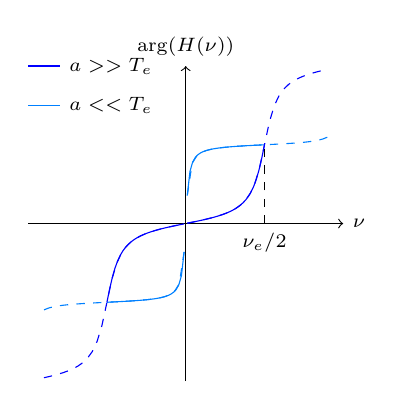
\begin{tikzpicture}
\begin{scope}[scale=2] 
\draw[->] (-1,0)--(1,0) node[right] { $\scriptstyle \nu$};
\draw[->] (0,-1) -- (0,1) node[above] {$\scriptstyle \text{arg}(H(\nu))$} ;

\draw[dashed,domain=0.01:0.9,color=blue!50!cyan,samples=30] plot (\x,{1/2 - 1/180*atan(0.1/2*1/tan(3.14*\x r))});
\draw[dashed,domain=-0.9:-0.01,color=blue!50!cyan,samples=30] plot (\x,{-1/2 - 1/180*atan(0.1/2*1/tan(3.14*\x r))});
\draw[domain=0.01:0.5,color=blue!50!cyan,samples=30] plot (\x,{1/2 - 1/180*atan(0.1/2*1/tan(3.14*\x r))});
\draw[domain=-0.5:-0.01,color=blue!50!cyan,samples=30] plot (\x,{-1/2 - 1/180*atan(0.1/2*1/tan(3.14*\x r))});
 

\draw[dashed,domain=0.01:0.9,color=blue,samples=30] plot (\x,{1/2 - 1/180*atan(10/2*1/tan(3.14*\x r))});
\draw[dashed,domain=-0.9:-0.01,color=blue,samples=30] plot (\x,{-1/2 - 1/180*atan(10/2*1/tan(3.14*\x r))});
\draw[domain=0.01:0.5,color=blue,samples=30] plot (\x,{1/2 - 1/180*atan(10/2*1/tan(3.14*\x r))});
\draw[domain=-0.5:-0.01,color=blue,samples=30] plot (\x,{-1/2 - 1/180*atan(10/2*1/tan(3.14*\x r))});

\draw[color=blue!50!cyan] (-0.8,0.75) node[right,color=black] {\scriptsize $a<<T_e$} --(-1,0.75) ;
\draw[color=blue] (-0.8,1)node[right,color=black] {\scriptsize $a>>T_e$} --(-1,1) ;
\draw[dashed] (0.5,0)node[below] {\scriptsize $\nu_e/2$}--(0.5,0.5);
\end{scope} 
\end{tikzpicture}
\end{center}
\end{frame}

\begin{frame}
\frametitle{Synthèse de filtres récursifs:Transformation Bilinéaire}
Comparaison analogique/numérique par la transfo bilinéaire.
\vspace{0.2cm}
\begin{columns}
\column{60mm}


\begin{center}
\begin{tikzpicture}
\begin{scope}[scale=2] 
\draw[->] (0,0)--(2,0) node[right] { $\scriptstyle \nu$};
\draw[->] (0,0) -- (0,1.5) node[above] {$\scriptstyle |H(\nu)|$} ;

%\draw (0.5,-0.4) node {$\frac{f_e}{2}$};

\draw[domain=0.065:1.9,color=blue!50!cyan,samples=30] plot (\x,{1/sqrt((10*\x)^2 + 0.1^2))});
\draw[domain=0:1.9,color=blue,samples=30] plot (\x,{1/sqrt((10*\x)^2 + 2^2))});

\draw[color=blue!50!cyan] (1.2,1.25)--(1.4,1.25) node[right,color=black] {\scriptsize $a<<1$};
\draw[color=blue] (1.2,1)--(1.4,1) node[right,color=black] {\scriptsize $a>>1$};
\end{scope}
\end{tikzpicture}
\end{center}


\column{60mm}

\begin{center}
\begin{tikzpicture}
\begin{scope}[scale=2] 
\draw[->] (-1,0)--(1,0) node[right] { $\scriptstyle \nu$};
\draw[->] (0,0) -- (0,1.5) node[above] {$\scriptstyle |H(\nu)|$} ;

%\draw (0.5,-0.4) node {$\frac{f_e}{2}$};

\draw[dashed,domain=-0.9:0.9,color=blue,samples=30] plot (\x,{abs(cos(3.14*\x r))/(sqrt((2*sin(3.14 *\x r))^2 + (10*cos(3.14*\x r))^2))});
\draw[domain=-0.5:0.5,color=blue,samples=30] plot (\x,{abs(cos(3.14*\x r))/(sqrt((2*sin(3.14 *\x r))^2 + (10*cos(3.14*\x r))^2))});
\draw[dashed,domain=-0.9:-0.1,color=blue!50!cyan,samples=15] plot (\x,{abs(cos(3.14*\x r))/sqrt((2*sin(3.14 *\x r))^2 + (0.1*cos(3.14*\x r))^2)});
\draw[domain=-0.5:-0.1,color=blue!50!cyan,samples=15] plot (\x,{abs(cos(3.14*\x r))/(sqrt((2*sin(3.14 *\x r))^2 + (0.1*cos(3.14*\x r))^2))});
\draw[dashed,domain=0.1:0.9,color=blue!50!cyan,samples=15] plot (\x,{abs(cos(3.14*\x r))/(sqrt((2*sin(3.14 *\x r))^2 + (0.1*cos(3.14*\x r))^2))});
\draw[domain=0.1:0.5,color=blue!50!cyan,samples=15] plot (\x,{abs(cos(3.14*\x r))/(sqrt((2*sin(3.14 *\x r))^2 + (0.1*cos(3.14*\x r))^2))});

\draw[color=blue!50!cyan] (0.6,1.25)--(0.8,1.25) node[right,color=black] {\scriptsize $a<<T_e$};
\draw[color=blue] (0.6,1)--(0.8,1) node[right,color=black] {\scriptsize $a>>T_e$};
\draw[dashed] (0.5,0)node[below] {\scriptsize $\nu_e/2$}--(0.5,0.5);
\end{scope}

\end{tikzpicture}
\end{center}

\end{columns}
\only<2->{
\vspace{0.2cm}
Contrairement aux deux méthodes précédentes, on comprime l'intégralité de la réponse en fréquence analogique sur $[0,\nu_e/2]$ $\rightarrow$ en numérique \textbf{Pas de repliement spectral} 
}

\end{frame}

\begin{frame}
\frametitle{Synthèse de filtres récursifs:Transformation Bilinéaire}
Bon comportement en amplitude, mais...
\vspace{0.1cm}
\[s = \frac{2}{T_e} \frac{1-z^{-1}}{1+z^{-1}}\]\\
\vspace{0.1cm}
\only<2->{
Si on passe en fréquence, 
\[2j\pi\nu_a T_e = \frac{2}{T_e} \frac{1-e^{-2j\pi \nu_n T_e}}{1+e^{-2j\pi \nu_n T_e}}\]\\
}
\only<3->{
\vspace{0.1cm}
\[ \rightarrow \nu_a = \frac{1}{ \pi T_e} \tan(\pi \nu_n T_e)\]
}
\only<4->{
\vspace{0.1cm}
Si je choisis une fréquence de coupure $\nu_{c,a}$ en analogique, la fréquence de coupure $\nu_{c,n}$ après la transformation sera différente... \only<5->{$\rightarrow$\textbf{ On pré-déforme les fréquences avant la transfo bilin.}}
}

\end{frame}

\begin{frame}
\frametitle{Transformation bilinéaire : Résumé}
\begin{center}
\begin{tikzpicture}
		\node[rectangle,draw,align=center] (I) at (1,0) {$H(s)$};
		\draw (1,-1) node[text centered] {\scriptsize Fct° trsf. analog.};
		\node[rectangle,draw,align=center] (D) at (4,0) {$H(s_d)$};
		\draw (4,-1) node[text centered] {\scriptsize Fct° trsf. prédef.};
		\node[rectangle,draw,align=center] (N) at (7,0) {$s = \frac{\displaystyle  2}{\displaystyle  T_e} \frac{\displaystyle 1-z^{-1}}{\displaystyle  1+z^{-1}}$};
				\draw (7,-1) node[text centered] {\scriptsize Transfo. Bilin.};
		\node[rectangle,draw,align=center] (B) at (10,0) {$H(z)$};	
		\draw (10,-1) node[text centered]{\scriptsize Rep. fréq. filtre num.};
		\draw[->] (I)--(D);
		\draw[->] (D)--(N);
		\draw[->] (N)--(B);
\end{tikzpicture}
\end{center}
\begin{enumerate}
\item<2-> On sélectionne une filtre analogique avec les bonnes propriétés en fréquence 
\vspace{0.2cm}
\item<3-> On prédéforme les fréquences en analogique avec $\nu_a = \frac{1}{ \pi T_e} \tan(\pi \nu_n T_e)$
\vspace{0.2cm}
\item<4-> On applique la transformation bilinéaire
\end{enumerate}
\end{frame}

\subsection{Résumé de la synthèse de filtre}
\begin{frame}
\frametitle{Résumé: Synthèse de filtres}
Synthèse de filtres = \textbf{Détermination des coefficients de la fonction de transfert/réponse impulsionnelle.}\\
\vspace{0.3cm} 
\only<2->{
\begin{columns}
\column{60mm}
\underline{Filtres non-récursifs}: \\
\vspace{0.1cm}
\begin{itemize}
\item<3-> Méthode des fenêtres
\vspace{0.1cm}
\item<4-> Méthode l'échantillonnage en fréquence
\end{itemize}

\column{60mm}
\only<5->{
\underline{Filtres récursifs}: 
\begin{itemize}
\item<6-> Approximation de la dérivée 
\vspace{0.1cm}
\item<7-> Invariance impulsionnelle
\vspace{0.1cm}
\item<8-> Transformation bilinéaire

\end{itemize}
}

\end{columns}

}
\end{frame}
\end{document}